\documentclass[a4paper,11pt,oneside,openany,uplatex]{jsbook}
%
\usepackage{graphicx}
\usepackage{amsmath,amssymb}
\usepackage{theorem}
\usepackage{bm}
\usepackage{ascmac}
\usepackage{subfigure}
\usepackage{multicol}
\usepackage{setspace}
\usepackage{mediabb}
\usepackage{float}
\usepackage{latexsym}
\usepackage{url}
\usepackage{cite}
\usepackage{layout}
\usepackage{verbatim}
\usepackage{wrapfig}
\usepackage{ascmac}
\usepackage{makeidx}
\usepackage{booktabs}
\usepackage{multirow}
\usepackage{algorithm}
\usepackage{algorithmic}


% \includeonly{evaluation}

% \usepackage[top=30truemm,bottom=30truemm,left=25truemm,right=25truemm]{geometry}
%\usepackage{times, mathptm}
%
\renewcommand{\baselinestretch}{1.0}
\renewcommand{\figurename}{Fig.}
\renewcommand{\tablename}{Table.}
\renewcommand{\headfont}{\bfseries}

\makeindex

\setlength{\textwidth}{150truemm}
\setlength{\fullwidth}{\textwidth}
\setlength{\oddsidemargin}{30truemm}   % 左余白
\addtolength{\oddsidemargin}{-1truein} % 左位置デフォルトから-1inch
\setlength{\topmargin}{30truemm}       % 上余白
\setlength{\textheight}{227truemm}     % テキスト高さ: 297-(30+30)=237mm
\addtolength{\topmargin}{-1truein}     % 上位置デフォルトから-1inch
\setlength{\voffset}{-0.55in}
\makeatletter
%
\def\thesis{Master Thesis}
\def\gakui{2014年度 修士論文}
\def\title#1{\def\title{#1}}
\def\daimoku#1{\def\daimoku{#1}}
\def\id#1{\def\id{#1}}
\def\department#1{\def\department{#1}}
\def\shozoku#1{\def\shozoku{#1}}
\def\author#1{\def\author{#1}}
\def\chosha#1{\def\chosha{#1}}
\def\submission#1{\def\@submission{#1}}
\def\teacher#1{\def\teacher{#1}}
%
\def\maketitlea{
\begin{center}
{\huge \thesis \par} 
\vspace{10mm}
{\huge \gakui \par} 
\vspace{10mm}
{\LARGE \daimoku \par}% 論文のタイトル部分
\vspace{10mm}
{\Large \title \par} %
\vspace{10mm}
{\Large \@submission \par} %
\vspace{15mm}
{\Large \shozoku \par} 
{\Large \id \chosha \par} % 学籍番号部分
\vspace{10mm}
{\Large 指導教員  \teacher \par}
\vspace{10mm}
{\Large \department \par}
\vspace{10mm}
{\LARGE \author}
\end{center}
%\par\vskip 1.5em
\clearpage
}
%
\daimoku{Multipath TCPによる経路切り替え手法を用いた \\ データセンターネットワークにおける \\ ショートフロー完結時間の改善}
\title{Improving the flow completion time of short flows in datacenter network
with path switching by Multipath TCP}
\date{\today}
\shozoku{東京大学大学院 \\ 工学系研究科 電気系工学専攻}
\department{The University of Tokyo \\ Graduate School of Engineering,
Department of Electrical Engineering and Information Systems}
\id{37-136482}
\chosha{藤居 翔吾}
\author{Shogo Fujii}
\submission{平成26年 2月5日 提出}
\teacher{関谷 勇司}

%%%%%%%%%%%%%%%%%%%%%%%%
\makeatother
%

\begin{document}
%
\pagestyle{empty}
\maketitlea


\begin{center}
{\large {\bf 要旨}}
\end{center}
クラウド型のサービスの性質により, 今日のデータセンターではデータセンター内のトラフィックが増大しており,
複数の経路を持つネットワーク環境を応用して, 通信性能向上を目指す取り組みがされている.
しかし, 様々なニーズを抱えるトラフィックが混在している中で, レイテンシ志向なサイズの小さいフローに対し,
既存のMPTCP実装では性能を劣化させる問題が報告されている.
そこで本研究では, この問題に対し, 並列分散処理アプリケーションが稼働しているクラスターPCのトラフィックを観測する事で, 単一NIC(Network
Interface Card)への通信集中によるキュー負荷の影響があることを検討し,
サイズの大きいスループット指向なロングフローとサイズの小さいレイテンシ指向なショートフローが一つのリンクに混在して通信を行っていることを明らかにし,
それによる通信性能障害が生じる技術的背景を考察した. 
そして, フローの指向毎に異なる通信経路を利用するレーンモデルを提案した. 
また, OSレベルから一つの通信を見た際に, そのフローの指向をフロー持続時間を用いて分類し, 経路の状況に合わせた経路切替手法を提案した. 
提案手法をOSに実装し, シミュレーションを用いた評価を行い, ロングフローとショートフローが混在する環境下で,
それぞれの指向毎に経路を切り替える制御を行うことで, ショートフロー通信を短縮化ならびに, ロングフローの通信性能を改善することを示した. 


\vspace{5mm}

\begin{center}
{\large \bf Abstract}
\end{center}
As increasing the amount of traffic in a datacenter by cloud service, the
effective network for utilization of massive computer clusters has been studied.
Recently, Multipath TCP(MPTCP) has been tackled this problem.
MPTCP can achieve the effective consumptions of the resources with multipath,
but a researcher reported MPTCP causes the delay of flow completion for short
flows in such a multipath network environment.
In this paper, I presented measurements of the distribute processing cluster
PCs and reveal impairment mechanisms that lead to that latencies, rooted in single
NIC(Network Interface Card) with intensive load traffic. 
I revealed there are both latency-oriented short flow and throughput-oriented long flow in a datacenter network. 
As the result, they lead to the performance impairment in flow completion time. 
In order to solve this problem, I proposed datacenter lane model to utilize different paths for each requirement of the flow. 
I developed the method of flow-classification for the orient and path-switching scheme to react the path condition with flow duration time, as approach just for end-node. 
I implemented these techniques to the end-node OS, and evaluated by simulation experiment. 
In my experiment, my proposals improve the performance for short flow in
shortening the FCT and long flow in increasing throughput with the control to separate the mixture traffic into both latency oriented flow and throughput-oriented one.

\clearpage

\frontmatter
\pagestyle{headings}
\tableofcontents 
\clearpage

\frontmatter
\pagestyle{headings}
\listoffigures
\clearpage


\frontmatter
\pagestyle{headings}
\listoftables
\clearpage



\mainmatter
\pagestyle{headings}

\chapter{序論}

\section{研究背景}
今日の一般家庭のインターネット接続環境が, ギガビット級の速度に達しようとしている中, 多様な端末がインターネットに接続できるようになり,
大量かつ多種多様なデータの取得が可能となった.
特にトラフィックデータ量の増加傾向は顕著で, 18$\sim$24ヶ月単位で総データ容量が2倍になるという予測がされている~\cite{IBM_rep}.
またFacebookでは, 300ペタバイト以上のデータ量を保有しており, 1日あたりに1ペタバイトのデータを解析している~\cite{presto}.
このように近年では, ビッグデータの活用が着目され, 例えばウェブ検索エンジン, SNS(Social Networking
Service)などのデータセンターを用いたクラウド型サービスにおいて, リアルタイムに近いレスポンスを返すような場面で使われ始めている.
そのようなクラウドサービスには近年, より高いユーザーエクスペリエンスが要求されており,
Amazonでは100[ms]の遅延により売り上げが1\%下がる, といった報告~\cite{amazon}があるように,
例えばeコマースサイトでの商品購入や,
インターネット広告のコンバージョンのようなユーザの意思決定へのレスポンス遅延の影響は深刻な問題である~\cite{customer_impact}.
そのため, 大規模データをより高速に処理することが求められており, データセンターではサーバ運用台数が増加の一途を辿っている.
そうした中で, 可用性, 計算性能, 低コストの三つの要件がデータセンターの抱える課題となっている~\cite{requirement}.
特に計算性能について, 大量の計算機資源から最大限の性能を引き出すためには,
従来の仕組みではデータセンター内トラフィックに対して一部の資源にトラフィックが集中する問題に対応できないため,
計算機資源を有効活用するための研究が盛んに行われている\cite{mapreduce, fattree,
dctcp, improving, detail, p_fab, synchro}.
そのようなスケーラビリティ拡大には, ネットワークトポロジー, アプリケーション, プロトコルに対する三つのアプローチがある.

ネットワークトポロジーを改良するアプローチでは, 近年データセンター内の通信帯域が1Gbpsから10Gbps, 40Gbps,
100Gbpsへと拡大していく中で, 従来の単純な二分木階層構造では,
データセンター内で発生するトラフィックに対して通信帯域を最大限割り当てることができない~\cite{fattree}.
そのため,
近年ではデータセンター内のトラフィックに対してスイッチを二段, 三段と少ない段数で構成し,
エンドノードから接続されるEdgeスイッチとそれらを集約するためのAggregationスイッチをより多く用いて接続することで, 
垂直方向には低く, 鉛直方向には大きく広がるトポロジーを提案している. 
これによって, データセンター内のトラフィックに対して通信帯域を有効利用することができる. 
また, データセンター内の通信においては, ノード間の通信経路が複数設けられており, 仮に一つの通信経路が切断されてしまったとしても,
残りの経路を用いて通信することができる, 可用性を持ち合わせたマルチパス環境を実現している~\cite{fattree}.
さらに, 近年のデータセンタートポロジーの動向として, 通信機器のコモディティ化があり, 特殊なデバイスや高価な機器を用いずに,
安価で汎用性のある機器を複数利用することで, 同等の性能を出そうと, 低コスト化を目指している. 

大量データの処理速度を改良するアプローチでは, データセンターの抱える巨大なデータの有効活用のために, 並列分散処理技術を用いることが一般的である. 
並列分散処理技術によって, 一つの処理を複数のサーバで同時並列で処理をすることで,
高スループットなデータ処理を実現しており, 大量の計算機資源から最大限の性能を引き出している. 
こうした並列分散処理技術ではpartition-aggregate計算モデルによって, 処理を細分化し, 各サーバに処理を割り当て, 結果を集約していき,
処理を完結させていく. 
こうした並列分散処理システムのアーキテクチャ上, 細分化された処理をそれぞれの処理サーバに割り当てる際, また計算結果を集約していく際に, 
サイズの小さいデータの通信が大量に発生し, データセンターネットワークの性能改善のボトルネックとなっている. 
MapReduce~\cite{mapreduce}等の並列分散処理フレームワークは,
これに従っており, 今日の大規模クラウドサービスにおいて必要不可欠である.

プロトコルを改良するアプローチでは, 
従来のTCPを拡張したMultipath TCP
(MPTCP)~\cite{mptcp}をデータセンターネットワークに用いる提案がされている~\cite{fattree}.
MPTCPを用いることにより, OSの制御によって複数のNIC(Network Interface Card), 複数の経路を同時に利用し,
スループットを向上させることが期待されている.
また, 近年のマルチパス環境を持つトポロジーにおいて, 一つの通信経路が切断された中でも,
一つのデータ通信の中で, 他の経路を使って途切れることなくデータ転送できる, 耐障害性を実現している. 
MPTCPでは, 従来のTCPと同様に, 3ウェイ・ハンドシェイク互いのコネクションを確立させ, その直後に互いの持っている他のIPアドレスを交換する. 
その後, サブフローを形成し, 複数の経路での通信をしていく. 
このためMPTCPの実装上, 比較的サイズの小さい通信では, サブフローを形成する前に通信が完了し, 結果的に一つの経路でのみ通信が行われることとなる. 

クラウド型サービスを実現するデータセンターネットワークにおいて,
並列分散処理アプリケーションによって大量に生成されたショートフロー通信が改善の課題となっている. \cite{improving}
実際, データセンター内でのトラフィックの内, 約80\%がショートフローであり, 並列分散処理の構造上,
ショートフロー通信時間が大規模計算処理高速化のための極めて重要な要素となっている. 

しかし, 既存のTCPを用いたクラウド環境では, このショートフロー通信の一部が大きく遅延する問題が報告されており,
既存のデータセンターネットワークを改善する上で, ショートフローの遅延の問題は深刻であると言える\cite{improving, rtt}.


\section{研究目的}
データセンターにおけるマルチパス環境でのショートフロー遅延の問題は並列分散処理性能の面で深刻な問題であり,
本研究は, 低レイテンシなネットワークによるコンスタントに性能の出せるデータセンターの実現を目指す.
そのために二つの手法を提案する. 

一つ目は, 異なる通信目的によって経路を切り替えるための通信レーンを複数設けるデータセンターモデルを提案する. 
これによって, 通信開始付近の経路については, 輻輳のない良好な通信環境である, ショートフローレーンで通信することができ,
その通信がショートフローであるならば, 遅延なく通信を終えることができる. 
比較的長い時間ショートフローレーンを占有するならば, ショートフローレーンからロングフローレーンへと通信経路を切り替え, 通信を行う. 
このモデルによって, ショートフローの遅延を抑え, ロングフローはショートフロー通信に干渉しない制御が実現できる. 

二つ目は, MPTCPを応用した通信経路切り替え手法を提案する. 
この手法によって, データサイズの小さいフローについては, ショートフローレーンを用いて遅延なく通信を完了させる. 
また各経路について, 通信状況を監視し, それぞれコストを計算することで, 通信経路を切り替える制御を実現する. 
この手法によって, 一つの経路に偏ることなく, それぞれの経路に均一に通信が割り振ることができる. 
さらにこの手法の実装には, Multipath TCPを応用して実現することで, OSベースで既存のアプリケーションに対して変更なく,
現実世界へ適用することが可能になる. 

\section{本研究の貢献}
本研究では, 提案手法を設計する指針となった取り組みについて, 二つの成果がある. 

一つは, MPTCPとTCPが互いに混在するような通信環境において, MPTCPがTCP通信に対して性能劣化を引き起こすという点である. 
主に通信経路の輻輳により, 通信開始時にパケットロスが生じることで遅延が生じることが分かり, 輻輳している経路を避け, 適切な経路を選択するためには,
コネクションを接続する時点で行う必要があることを示した. 

二つ目は, 実際の並列分散処理アプリケーションがどのようなトラフィックを生成するのか解析を行った. 
この解析によって, 並列分散処理アプリケーション特有のトラフィックを明確にし, 
それによって汎用的なネットワーク機器を用いたデータセンターにおけるショートフロー遅延が生じる背景について, ボトルネックとなりうるネットワーク環境を検討し,
その原因を示した.

本研究で提案したネットワークモデルと通信経路切り替え手法は, サイズ小さいショートフロー通信における遅延を抑えることができた. 
本研究の成果により, 通信時間の長いサイズの大きいフローについては, MPTCPにより高スループット化を実現した. 
また, 既存のデータセンター内通信では, サイズの大きいフローの影響を受け, 通信時間の短いショートフローが遅延してしまっていたのに対し, 本店案手法によって,
特に遅延していた, 下位10\%のフローに対して, 通信時間の短縮かを実現できた. 
さらに, 本研究の提案手法では, MPTCPを応用することによるOSベースの手法であるため,
OSを書き換えるだけで利用することができるという実現可能性が高い手法としての利点がある. 

\section{本研究の構成}
本論文の構成は以下の通りである. 
第\ref{chapter:related_work}章では, 低レイテンシなデータセンターネットワークに関する研究について, アプローチする場所ごとに述べ,
データセンターネットワークが抱えている要求案件と 既存研究手法の課題を議論する. 
第\ref{chapter:datacenter_network}章では, データセンターが構成する技術要素と抱えている技術的課題を述べ,
提案手法の位置付けを示す. 
第\ref{chapter:motivated_work}章では, 既存技術の抱える課題やこれまで報告された問題点を, 再現実験により改めて見直すことにより,
提案手法の設計する上での指針を示す. 
第\ref{chapter:proposal}章では,
複数のレーンを用いたデータセンターモデルとMPTCPを応用した通信経路切り替えアルゴリズムを併用した本研究のショートフロー改善手法を提案し, 既存研究との差異を明確にすることで, 本研究の位置付けを明らかにする. 
第\ref{chapter:evaluation}章では, 実際のデータセンターネットワークを想定したトラフィックに対して, 提案手法と既存手法を比較,
また提案手法の性能評価実験の方法と結果について述べる. 
第\ref{chapter:consideration}章では, 実験の考察と実験結果をもとにした提案手法の応用に関する考察を述べる. 
最後に, 第\ref{chapter:conclusion}章で, まとめと今後の課題について述べる. 



\chapter{関連研究}
\label{chapter:related_work}
本章では, これまでに報告されている複数経路利用によるフロー完結時間短縮化技術について簡潔に述べ, その優位性や問題点を示す.
大量のネットワーク機器により構成されており, 短時間で大量のデータをの処理を行うデータセンターネットワーク環境において,
リクエストに対するレスポンスの高速化によるより良いユーザエクスペリエンスの向上が求められている. 
本章では, これまでに報告されているデータセンターにおける低レイテンシなネットワークに関する研究について述べる. 
既存の研究では, キュー長の縮小, 再送処理の高速化, ショートフローの優先付け, 複数経路の利用の4つの技術を用いることで実現しており,
4つの分類ごとにその特徴や課題について考察する. 
そして, 本研究の位置付けを示す. 



\begin{table}[t]
\begin{center}
{\footnotesize
\begin{tabular}{c|c|c|c|c|c|c|c}
\hline
\multicolumn{2}{c|}{\multirow{2}{*}{Categories}} &
\multirow{2}{*}{Proposals} &
\multicolumn{2}{c|}{Objectives} & 
\multicolumn{3}{c}{Modifications to} \\\cline{4-8}
\multicolumn{2}{c|}{ } &  & FCT & deadline & TCP & Switches & applications \\
\hline
\multicolumn{2}{c|}{\multirow{2}{*}{Redcing queue length}} &
DCTCP & mean & $\times$ & $\surd$ & $\times$ & $\times$ \\ \cline{3-8}
\multicolumn{2}{c|}{ } & HULL & mean & $\times$ & $\surd$ & $\surd$ & $\times$
\\ \hline

\multirow{6}{*}{\parbox{8zw}{Prioritizing flows basd on}} &
\multirow{4}{*}{\parbox{6zw}{Flow deadlines}} & ${\rm D^3}$ & none &
 $\surd$ & $\surd$ & $\surd$ & $\times$ \\ \cline{3-8}
 
 & & PDQ & none &
 $\surd$ & $\surd$ & $\surd$ & $\times$ \\ \cline{3-8}
 
 & &${\rm D^2TCP}$ & tail &
 $\surd$ & $\surd$ & $\times$ & $\times$ \\ \cline{3-8}
 
 & & MCP & tail &
 $\surd$ & $\surd$ & $\times$ & $\times$ \\ \cline{2-8}

 &\multirow{2}{*}{\parbox{6zw}{Application assignment}} & pFablic &
 \parbox{3zw}{\strut{}mean \& tail\strut} & $\surd$ & $\surd$ &  $\surd$ &
 $\surd$
 \\
 \cline{3-8}
 
 & & \multirow{2}{*}{Detail} & \multirow{2}{*}{tail} &
\multirow{2}{*}{$\surd$} & \multirow{2}{*}{$\surd$} &
\multirow{2}{*}{$\surd$} & \multirow{2}{*}{$\surd$} \\ \cline{1-2}

\multicolumn{2}{c|}{\multirow{2}{*}{Exploiting multipath}} & & & & & \\
\cline{3-8}

\multicolumn{2}{c|}{ } & RepFlow & \parbox{3zw}{\strut{}mean \& tail\strut} &
$\times$ & $\times$ & $\times$ & $\surd$ \\ \hline

\multicolumn{2}{c|}{\multirow{3}{*}{Accelerating retransmissions}} & DIBS & tail
& $\times$ & $\surd$ & $\surd$ & $\times$ \\ \cline{3-8}

\multicolumn{2}{c|}{ } & FastLane & tail
& $\times$ & $\surd$ & $\surd$ & $\times$ \\ \cline{3-8}

\multicolumn{2}{c|}{ } & CP & tail
& $\times$ & $\surd$ & $\surd$ & $\times$ \\ \hline

\end{tabular} 
}
\caption{An overview of low latency datacenter networking proposals}
\label{table:proposal_list}
\end{center}
\end{table}

\section{キュー長の縮小}
レイテンシの大きいデータセンターネットワークの主な原因はキューイング遅延である\cite{dctcp}. 
報告された解析結果\cite{dctcp}によると, ネットワーク全体のトラフィック量が比較的小さく, 大きな輻輳が発生していない環境においても,
ショートフローのフロー完結時間の大部分がキューイング遅延に依存する. 
キューイング遅延を減らし, 遅延を改善するための一つの手法として, キュー長の縮小がある. 

スイッチのキュー長を減らし, バッファの占有を抑えることにより, 遅延を改善するアプローチは最も直接的な手法である. 
高速に処理のできない汎用的なスイッチではバースト性のあるトラフィックに対して, バッファを多く用意することで対応している. 
データセンターネットワークでは基本的に帯域遅延積が小さく, バッファが大きいと通信性能に影響が出る. 
既存のTCPの服装制御では, ロングフローがバッファを使い切るまで通信しようとし, それにより大きなキューイング遅延が生まれ,
ショートフローの通信性能に影響が出る. 
そのため, キューイング遅延を抑えるために, スイッチのバッファを小さくし,
新しい帯域制御手法や輻輳検出のための仕組みがエンドノードとスイッチに対して必要となる. 

DCTCP\cite{dctcp}とHULL\cite{hull}はスイッチバッファの占有率を持続的に低く抑え, 遅延を抑える為に提案された手法である. 

\subsection{DCTCP}
DCTCP(Data Center TCP)\cite{dctcp}はデータセンターネットワーク内の遅延問題の解決を目指した初めての取り組みである. 
Alizadehら\cite{dctcp}は実際に稼働しているデータセンターのトラフィックを観測, 1ヶ月分のトラフィックデータの解析を行い,
データセンターネットワークが生成するトラフィックの特徴を考察した. 
その結果, データセンターのトラフィックの大部分が遅延指向なショートフローであることを示し,
ロングフローによってバッファが占められた中継されるスイッチの影響でそれらのフローが大きく遅延することを示した. 
これらの観測結果が動機となり, 著者たちはスループット性能を大きく損なうことなく,
バッファの占有を抑える為の輻輳手法としてDCTCPという新しいトランスポートプロトコルを提案した. 

DCTCPは汎用的なスイッチにも広く実装されているExplicit Congestion
Notification(ECN)による輻輳通知の機能を用いている.
バッファ占有のしきい値をあらかじめ設定しておき, それを超えると,
スイッチがパケットのTCPヘッダーのECNエコーフラグを用いてエンドノードに明示的に通知する.
この情報を用いてサーバホストはTCP遅延ACKにECNエコーフラグを加えクライアントホストに知らせる. 
そしてクライアントホストでは, ECNマークされたパケットの割合によって, スイッチバッファの状態を推定し, ウィンドサイズを抑える. 
その結果, キュー溢れが起こる前に輻輳を回避することができ, バッファ占有を抑えることができる. 
DCTCPは既存のTCP実装に対して, 30行の変更を加えるだけで利用することができ, 今のインフラに対して容易に展開することができる. 
DCTCPはテストベッド環境においてFCTを大きく改善することができ, 特にテール部分について,
99パーセンタイルFCTをTCPの40\%以上短縮化することができた. 


\begin{figure}[t]
    \begin{center}
    
\includegraphics[autoebb, width=200pt]{./img/test.pdf}
    \caption{The control loop in DCTCP(DCTCPの制御の流れの模式図, キューの様子,
    しきい値を超えた時の通知の仕組み)}
    %\ecaption{The control loop in DCTCP}
    \label{fig:dctcp_control}
    \end{center}
\end{figure}

\subsection{HULL}
HULL(High-bandwidth Ultra-Low Latency)\cite{hull}はDCTCP実装をベースに追加で用いる手法であり,
さらなるキュー長の縮小のためのすべてのポートのキュー状態の推定を目的としたものである. 
HULLは直接的にキュー長の様子を通知するDCTCPとは異なり, 通信利用帯域によるリンク利用率を基にした輻輳通知手法である. 

HULLではリンク利用率を用いたファントムキューという仮想キューを利用している. 
これは, バッファ処理自身のオーバーヘッド影響を考慮せず,
実際の物理リンクよりも低い通信レートでの仮想リンクにおけるキューイングの様子をシミュレートすることによって算出される. 
ファントムキューがしきい値を上回った場合, DCTCPと同じECNを用いた通知機構を用いて, ウィンドウサイズの調整を行いキュー長を抑える. 
ファントムキューは物理リンクよりも低いレートにおいてシミュレートされているため, よりレートの高い実際の環境におけるバッファではより小さく保つことができ,
キューイング遅延の影響がより小さくなる. 
著者は平均値, 99パーセンタイル値のFCT共にDCTCPの10倍以上, TCPの40倍以上改善することができたことを示した. 
しかしFCTの改善のトレードオフとして約10\%の利用帯域の減少も生じていることも示した. 

\section{再送の高速化}
データセンターネットワークの遅延を抑える為の手法として, パケットロスによる遅延に対して改善を行う手法がある. 
通常TCPでは, パケットロスが起こった場合, それを検知するためのタイムアウト時間RTO後に再送制御を行う. 
一般にRTOはエンドノード間のRTTよりも非常に大きな値を設定するため, RTOによって不必要な時間分だけ待たなければならない. 
先行研究として提案された手法では, RTOを小さくする, あるいはRTOによる再送制御を無視し,
明示的にエンドノードに対してパケットロスが起こったことを通知することで, 再送遅延の短縮化を実現している. 

ショートフローとロングフローの両方が共存している場合, パケットロス, 再送制御が起こることは避けられれない. 
パケットロス自体は頻繁に起こるわけではなく, その割合も小さいため, 再送制御による遅延を改善することはテール部分の遅延の改善に対して大きく貢献する. 
TCPでは, 基本的にはショートフローのFCTはRTOよりも短いため, パケットロスが起きた場合の影響は非常に大きい. 
RTOはパケットロスを検知するためにエンドノード間の最大RTTよりも大きな値を設定するが,
例えばアプリケーション性能に依存するショートフローにとって, そのFCTがデッドラインを満たすためにはRTOは非常に大きい. 
またTCPの服装制御では, パケットロスが起こった際に, ウィンドウサイズが減少され, フローを完結するためにより多くのラウンドトリップが必要となる. 

先行研究では, この問題を解決するために, 二つの観点からアプローチしている. 
DIBS\cite{DOBS}ではパケットロスが起こった際, その混雑しているポートとは異なる他のポートをランダムに選択,
パケットをリダイレクトし再送制御を行う. 
また, FastLane\cite{fastlane}, CP(cutting
Payload)\cite{cp}では高速に明示的な通知をエンドノードにおこうことで, 再送制御を高速化する. 

\subsection{DIBS}
Detour-Induced Buffer Sharing\cite{DIBS}では, アイドル状態のネットワーク資源を利用し,
ホットスポットでのバーストトラフィックを緩和させる. 
スイッチがパケットロスをしなければならない時, 本来転送しなければならないポートとは異なる他のポートをランダムに選択し, パケットを転送する. 
これにより3つの効果を生み出すことができる. 
\begin{enumerate}
\item 他のパスに転送されることでより多くのホップ数を必要とするかもしれないが, 服装が起こっているホットスポットを避けることができる. 
\item 転送したパケットがループバックしてきた際に, 本来転送するべきポートのバッファが占有されていないパケットロスが怒らない状態であればそちらに転送する. 
\item そのパケットのTTLに達するまでに, アイドル状態のパスを見つけられなかった際には, パケットは破棄される. 
\end{enumerate}
複数の等価コストのパスをもつデータセンターネットワークの性質上, 迂回経路によって大部分のパケットロスを抑えることができる. 
また, アイドル状態のパスを見つけられない可能性はデータセンターでは低いが, その際にはタイムアウトや再送制御が行われる. 

\subsection{FastLane, CP}
FastLane\cite{fastlane}とCP\cite{cp}は再送制御の高速化のための明示的なパケットロスの通知を生成する. 
それにより, 再送制御を起動させるまでのオーバヘッドをRTO時間から1回分のラウンドトリップへと減少させる. 

FastLane\cite{fastlane}は, パケットロスを引き起こしたスイッチで検出し, 直ちにエンドノードへ通知を行う. 
CPUのオーバーヘッドを抑えるために, ロスを引き起こしたパケットのIPアドレスをスワップし, エンドノードへ通知する. 
これにより, エンドノードはどのフローでロスが発生したかを素早く知ることができる. 
また, 通知するためのトラフィックに対し, 通信帯域の制限(bandwidth cap)をすることで,
ネットワーク全体の帯域オーバーヘッドを抑えることができる. 
一方, CP\cite{cp}は通知のために新しいパケットヘッダーを用いる. 
パケットロスが起こった時に, ペイロードの大きいパケットについてはペイロード部分を取り除く. 
通知を受けたノードは, ヘッダーを見てペイロードが除去されていることを認識し, 
SACKのようなピンポイントでのACKによって再送制御を呼び出す. 
FastLaneもCPもどのトランスポートプロトコルと互換性を持つ手法である. 

\section{ショートフローへの優先付け}
ショートフローのFCTを改善するために遅延を抑える手法として, 優先制御がある. 
どのパケットも同じ扱いをするTCPとは異なり, ショートフローに対しては優先度を高く設定し,
他のキューイングされているパケットよりも前に処理されるような優先制御が行われ, それによりショートフローのFCTが大きく改善される. 
フローの優先付けには二つの方法がある. 
一つは, アプリケーションによって明示的に優先度を定められ, 優先度を割り当てられる手法\cite{pfabric, detail}. 
他方は, 今日のデータセンターの扱うアプリケーションが暗黙的に定めるデッドライン情報を用いて優先度を割り当てる手法である. 
いくつかのアプリケーションでは各フローに対しておよそ200ms$\sim$300msのデッドラインを満たす要求があり, 優先制御によりそれを実現する. 
また, そうしたデッドラインが明示的に定められないものについては, レスポンス時間を保証するために用いられる\cite{mcp, pdq, d2tcp, d3}.
そのため, ネットワーク内のスケジューリングによるフローの優先付けは既存のトランスポート層,
データリンク層のプロトコルを改良することで効果的な手法が実現される. 

ロングフローであるかショートフローであるかに依らず, どのパケットも公平に扱おうとする他のアプローチでは,
インターネットにおける通信公平性を保証する一般的な設計指針である. 
しかし, データセンターネットワークでは, ロングフローによるショートフロー通信性能の劣化を引き起こすという状況がある中で, こうした考えは,
不公平であるという議論もある\cite{mcp, pdq, d2tcp, d3}.
そうした不公平性の問題を解決するために優先制御手法が提案されているが, 大きく2種類の情報を使う手法に分類することができる. 
一つは, フローのFCTのデッドラインによって優先度を決める手法. 
他方はアプリケーションによって明示的な優先度を設定される手法がある. 

\subsection{デッドラインベースの優先付け}
\subsubsection{$D^3$}
$D^3$ (Deadline Driven Delivery)\cite{d3}はデッドラインベースの優先制御手法である. 
$D^3$では, フローのデッドラインを満たすために十分である帯域を算出し,
割り当てることによってネットワークリソースの最適な配分ができるという考えに基づいている. 

Wilsonら\cite{d3}は, サーバとクライアントでインタラクティブな通信を必要とする多くのアプリケーションは,
そのアプリケーションフローを生成する処理ノードによってデッドラインが定められていると述べており, このデッドライン情報を用いることで,
$D^3$はデッドラインまでに通信を完了できる最小のレートを算出し, パケットのヘッダー情報として追加しておく. 
それにより, フローは中継するすべてのスイッチに対して必要な帯域を要求することができる. 
スイッチはACKパケットによってそのリクエストに対する予約帯域をエンドノードに通知する
そしてクライアントノードはその通知に従って送信レートを調整する. 

$D^3$が適用されるスイッチでは, その時間で通信を行っているフローに基づいて帯域の割り当てが行われる.
計算, メモリー容量を抑えるため, スイッチによる帯域割り当ては, FCFS(first-come-first-serve)に基づいて実行される. 
そのため, すべてのフローに対して要求を満たすための帯域が不十分な状況であれば, 先着順で初めのいくつかのフローしか満たせない可能性もある. 

\subsubsection{PDQ}
$D^3$のFCFSスケジューリングは十分なパフォーマンスを引き出せない場合がある. 
十分にパフォーマンスが引き出せない状況について, Fig\ref{fig:fair_share}に示す. 
こうした公平性の考えがPDQ(Preemptive Distributed Quick)フロースケジューリングの設計指針となっている. 
PDQは$D^3$のスケジューリングに対して横取りスケジューリングをすることを許可し,
デッドラインを素早く満たせるフローについては積極的に帯域を割り当てるような制御を行う. 

PDQでは, デッドラインが短いフローから, サイズが短いフローから, の二つの規律に従ってスケジューリングを行っている. 
このスケジューリングを実現するために, 分散スケジューリングレイヤーによって, 他のスイッチと連携を取り, 安定的な帯域割り当ての決定へと収束させる. 
PDQによるスケージュリングはFIFO droptail キューを用いて近似的に実現している. 
シミュレーションによる実験では, 現実世界でのトラフィックでの検証を行い, $D^3$に対して, 平均FCTを30\%以上改善することができたと報告している. 

\begin{figure}[t]
    \begin{center}
    
\includegraphics[autoebb, width=200pt]{./img/test.pdf}
    \caption{Fair-share(e.g. DCTCP)and $D^3$ are sub-optimal in meeting
    deadline FCTベースでの通信の公平性についての図, グラフ)}
    %\ecaption{The control loop in DCTCP}
    \label{fig:fair_share}
    \end{center}
\end{figure}

\subsubsection{$D^{2}TCP$, MCP}
$D^{2}TCP$\cite{d2tcp}, MCP\cite{mcp}では, フローのTCP ウィンドウサイズを調整することで, デッドラインを満たす制御を行う. 
いずれの手法も, ECNによって服装状態を推定するDCTCP\cite{dctcp}を基にした手法で,
DCTCPの手法にフローのデッドライン情報を考慮に入れて, 優先制御を実現している. 

$D^{2}TCP$はガンマ補正関数を用いてデッドラインを満たすTCPウィンドウサイズに調整する. 
具体的には, デッドラインに近いフローほど, より多くのウィンドウサイズが割り当てられるような制御がされる. 
MCP\cite{mcp}はさらにもう一歩先に進んだ手法となっており, 通信が開始した直後にデッドラインを満たすようなウィンドウサイズの調整が行われる. 
具体的には, ECNベースの輻輳制御が行われ, 長期的なパケットごとの平均遅延時間を最小にする最適化問題としてアルゴリズムが実装されている. 
Chenら\cite{mcp}は最適なウィンドウサイズの割り当てを凸計画問題として解き, 数値評価によって提案した近似アルゴリズムの有用性を示している. 


\subsection{アプリケーションベースの優先付け}
\label{subsec:ap_priority}

\subsubsection{DeTail}
Detail\cite{detail}はテールFCTの改善を目的としたクロスレイヤーフレームワークである. 
Zatsらはロングテールなレイテンシを持つFCTとなる二つの主な原因を示し, それらを低減する二つの手法を提案した. 
原因の一つは, それぞれのフローの中に優先度がないことである. 
一時的な輻輳状態の際, ロングフローの継続的な通信のためショートフローが十分なデータ量が通信できなくなり, 大きく遅延するフローが発生する. 
DeTailでは, 近年標準化されたPFC(Priority Flow Control)によるQoS制御によって, データリンク層においてこの問題を解決する. 
PFCは近年のL2スイッチには実装されており,
輻輳時に優先度の低いフローについて一時的に通信を止めることによる優先制御をスイッチからエンドノードに対して通知することで実現可能である. 

二つ目の原因は, ネットワークレイヤーにおける不均一なロードバランシングである. 
現在実装されている, ハッシュベースのロードバランス手法では, 輻輳が発生していない経路が存在しているにもかかわらず,
ロングフローとショートフローが同一の経路を選択する可能性がある. 
DeTailでは, 各経路の通信状況に適応させるマルチパスロードバランス手法($\S$\ref{subsec:u-multipath})によって,
この問題を解決している.

\subsubsection{pFabric}
多くの手法が様々な仕組みを組み合わせた複雑なシステムによって遅延の改善を目指してきたが, 提案したpFabric\cite{pfabric}では,
最小限のシステムによって問題の解決を目指している. 
pFabricの設計指針は, 優先制御による利得を最大限に引き出すことである. 
Alizadehらは, フローによって通信レートを差別化する手法は広く提案されているが, それらは効果的でなく, 実装も難しく,
そうした送り手側の通信レートの制御に代わり, スイッチにおけるショートフローの優先度付けのみで十分有効であると述べている.

pFabricでは, デッドラインが短いフローや, ユーザエクスペリエンスに大きく関わるフローについてはヘッダーの優先値を設定しておき,
中継スイッチのキューにおいて, 優先値の昇順で処理を行っていくことで, 優先度の高いフローが先に処理されていくような制御を実現している. 
さらに, スイッチのバッファは非常に小さく設定しておき, 容易にバッファの占有, パケットロスを引き起こさせる. 
ns-2でのシミュレーションでは, pFabricは平均, テールFCT共に理論値に近い値を達成している. 

\subsection{複数経路の利用}
\label{subsec:u-multipath}
4つ目の手法は, データセンターに内在する複数の経路を利用することである. 
多くのネットワークトポロジーでは, サーバ間通信の等価な通信経路が複数存在している. 
既存のマルチパスを活用した手法として, ECMP(Equal Cost Multi-path)がある. 
これは,  フローの5-タプルを用いてハッシュベースに経路を選択する手法であり, 通信トラフィックを準最適化する. 
マルチパス環境において, 輻輳のしていない経路を選択することで, キューイング遅延の影響を避けることができ,
様々なマルチパスロードバランシング手法が提案されている. 

\subsubsection{DeTail}
\ref{subsec:ap_priority}節で述べたように, DeTail\cite{detail}では, マルチパス環境で,
ネットワークレイヤーの通信経路に適応させたロードバランシング手法によって, 複数の経路をより効率的に活用することができる. 
リンクレイヤーでの優先付けと併せて, Fig. \ref{fig:detail_crosslayer}にこれら二つの手法から構成されているクロスレイヤーによる
DeTailのシステムを示す. 

特にDeTailのロードバランシングでは, パケットごとに制御が行われ, パケットがスイッチに到着したときに, 最小経路の中で,
最も利用率の低い経路を選択して転送される. 
通信している経路が輻輳状態になったら, PFCによるポーズ通知がすぐに送られ, 経路変更のトリガーとなる. 
アイドル状態の経路が存在しない場合, そのフローの通信が一時的に停止する.
DeTailではパケットごとに制御行われるため, それぞれのパケットを監視することは難しく, パケットの順序が入れ替わった場合の処理については,
既存のTCPに一任することとなる.
\begin{figure}[t]
    \begin{center}
    
\includegraphics[autoebb, width=200pt]{./img/test.pdf}
    \caption{DeTail's cross-layer design DeTailのクロスレイヤーで作用する仕組み}
    %\ecaption{The control loop in DCTCP}
    \label{fig:repflow_scheario}
    \end{center}
\end{figure}



\subsubsection{RepFlow}
これまでの遅延改善手法は, スイッチ, エンドノード, ネットワークスタック, あるいはネットワークファブリックそのものに対して変更が必要だった. 
RepFlow\cite{repflow}では, スイッチやエンドノードのカーネルに対する変更なしで,
ショートフローを複製し各経路に転送することでFCTの改善を目指す, 単純で効果的な手法である. 

RepFlowは, 例えばFatTreeトポロジー\cite{fattree}のような複数の経路が存在するネットワークでの経路の多様性に着目している.
バースト性のあるトラフィックによる一時的な輻輳状態やECMPによるハッシュの衝突は, 基本的には場所, 時間についてランダムに発生するものである. 
結果的に, 異なる経路における輻輳の度合いは統計上独立であると考えることができる. 
RepFlowでは, 複製されたフローと元のフローは高い確率で異なる経路を通り, その両方のフローがキューイング遅延が起こる可能性は小さい. 
Fig. \ref{fig:repflow_scheario}にホットスポットを回避できるシナリオを示す. 

データセンタートラフィックの特徴として,
90\%以上がショートフロー($leq$100KB)で全体のデータ量のおよそ5\%のみの割合である\cite{dctcp,
pfabric}ことからショートフローの影響はとても小さいと考えることができる. 
さらに, RepFlowは他のトランスポートプロトコルとの互換性があり,
既存のTCPだけでなくDCTCP\cite{dctcp}に対しても適用することができる. 
Xuらはシミュレーション実験によってRepFlowの性能を評価し,
FCTの平均値と99パーセンタイル値の50\%$\sim$70改善することができたことを示した. 
\begin{figure}[t]
    \begin{center}
    
\includegraphics[autoebb, width=200pt]{./img/test.pdf}
    \caption{An example to understand RepFlow:RepFlowがうまく作用するシナリオ例}
    %\ecaption{The control loop in DCTCP}
    \label{fig:repflow_scheario}
    \end{center}
\end{figure}
% 
% \section{プロトコルに対するアプローチ}
% 2011年にCostinらによって, MPTCPを用いたデータセンターネットワークモデルが提案された~\cite{improving}.
% 近年の大規模計算資源を有効活用するために提案されたネットワークトポロジーでは,
% 高性能なデバイスや特殊な機器を必要とせず, 汎用的なネットワーク機器のみを用いてデータセンター内のエンドノード同士の通信に経路が複数用意されている.
% 既存の取り組みでは, 通信に使わない経路をセカンダリ経路として利用することで, 耐障害性を持たせていたのに対し, 提案されたデータセンターモデルでは,
% MPTCPを用い複数経路を同時に利用する事で, 耐障害性を保ちながら, 帯域を最大限利用する事を可能にした.
% また, 様々なトポロジーにMPTCPを適用することで, 従来のTCPよりも高いスループットが出せることを示した.
% しかし, MPTCPとSingle path-TCPが混在する環境において, Single
% path-TCPで行われるサイズの小さいフロー($\leq70KB$)のフロー完結時間に着目すると, 従来のSingle
% path-TCPのみのネットワーク環境よりも時間がかかるという問題点があった.
% 現状のMPTCPの実装では, サイズの小さいフローにおいてはサブフローを形成する前に通信が完了するので, MPTCPとSingle
% path-TCPが混在する環境は十分起こりうるものである\cite{mptcp_ana}.
% 
% 
% \section{スイッチに対するアプローチ}
% 2012年にZarsらによって, 複数レイヤー間でトラフィックを監視し,
% しきい値を設定することによるフロー完結時間の短縮化技術を提案した~\cite{detail}.
% 今日のデータセンター内ネットワークのような, サイズの異なるフローが混在するネットワークにおいては, サイズが小さいフローがサイズの大きいフローに圧迫され,
% 伝送遅延が大きくなる問題があったが, この提案手法では, データリンク層からアプリケーション層までの各層が,
% 相互にトラフィックを監視する機能をスイッチに実装し, 優先度をつけ, バッファサイズを調整することで, フロー完結時間の劣化を抑えることを可能にした.
% しかし, 実験ではClick~\cite{click}を用いて実装を行っており, 現実世界での全てのネットワーク機器の置き換えが必要となるので, 実現は難しい.
% 
% \section{アプリケーションに対するアプローチ}
% 2014年にH. Xuらによって, 通信可能な経路の数だけソケットを複製し, 通信環境が最も良い経路のフロー完結時間を採用することで,
% フロー完結時間を短縮化する技術を提案した\cite{repflow}.
% 今日のデータセンターでは, データセンター内のノード間の経路が複数存在し, それらに対して例えばECMPのようなハッシュベースの経路選択を行うと,
% 通信環境の悪い経路を選択する可能性がある.
% この提案手法では, スイッチやノードのOSに対しての変更を必要とせず, 極めて単純な仕組みによって, フロー完結時間の短縮化を実現している.
% しかし, 最もフロー完結時間が短かったもの以外のフローに対しては, ノード間の通信にとって無駄なものとなり, ネットワーク全体の通信量増加による,
% 新たな輻輳を発生させる.
% また, 比較的サイズの小さいフローのみこの手法は有効であり, サイズの大きいフローに対しては, 従来の通信をよりも時間がかかることが理論的に示されている.
% そのため提案手法では, 事前にフローサイズを把握しておき, 提案手法を適用するか否かを判断する必要があるため, アプリケーションに対して変更が必要となり,
% これを現実世界への適用を考えると, すべてのアプロケーションに対して変更が必要となり, 提案手法の実用化は困難であると言える.





\section{本研究の位置付け}
これまでの関連研究を踏まえて, 近年のデータセンターネットワークに対して, 以下のような要件が考えられる.
\begin{itemize}
  \item 大規模計算機を有効活用するトポロジーの利用
  \item 分散処理の際に発生する大量のサイズの小さいフローの送信時間の短縮
  \item 特殊な実装やデバイスを用いず, 汎用的でシームレスな運用の実現
\end{itemize}
本研究ではこれらの要求案件を満たす, データセンターでのショートフローの改善手法を提案する. 


\chapter{データセンターネットワーク}
\label{chapter:datacenter_network}
本章では, データセンターネットワークを構成する技術に関して, その概要を述べる.

\section{トポロジー}
従来のデータセンターモデルでは, エンドノードがEdgeスイッチにつながり,
これらのスイッチがAggregationスイッチに集約され,
coreスイッチに接続するといったように, 階層的にトポロジーを形成していた~\cite{fattree}.
このような単純な階層構造を持つトポロジーは, トラフィックの大部分がデータセンター外の通信には有効であった.
しかし, 今日のようなデータセンター内で生じるトラフィックが大半を占める場合, 帯域の割当が適切でなくなる.
このような, データセンター内のトラフィックが主であれば, 階層型のトポロジーはボトルネックを引き起こす可能性がある.
近年の研究~\cite{fattree,bcube,vl2}では, トラフィックがデータセンター内に集中した時の問題を, 物理的なアプローチとして,
トポロジーを工夫する事で解消を試みている.

Fig.\ref{fig:fattree}のように, FatTree~\cite{fattree}では, Coreスイッチを複数用いる事で,
物理パスの最大帯域を供給する.
また, 比較的狭い帯域の経路と汎用的な性能のスイッチを多数用いる.

このようなトポロジーを用いる事で, データセンター内のトラフィックに対し, 帯域を十分に使う事ができる.
しかしこのような密な配置により, 複数の経路が形成され, ルーティングをどのように決定すべきかという問題も生じる事となる~\cite{improving}.
例えばFig.\ref{fig:fattree}のようなFatTreeトポロジーでは, 4通りの経路が考えられる.
これら複数の経路をリンクエラー時の冗長性を持たせる目的だけでなく, 性能向上に活用することが求められている.

\begin{figure}[h]
    \begin{center}
    \includegraphics[autoebb, width=350pt]{./img/hierarchy_topology.pdf}
    %\caption{階層型ネットワークトポロジー}
    \caption{Hierarchical network topology}
    \label{fig:hierarchical}
    \end{center}
\end{figure}

\begin{figure}[h]
    \begin{center}
    \includegraphics[autoebb, width=350pt]{./img/fattree_topology.pdf}
    %\caption{FatTreeトポロジー}
    \caption{Fattree topology}
    \label{fig:fattree}
    \end{center}
\end{figure}

\begin{figure}[h]
    \begin{center}
    \includegraphics[autoebb, width=350pt]{./img/bcube.pdf}
    %\caption{BCubeトポロジー}
    \caption{BCube topology}
    \label{fig:bcube}
    \end{center}
\end{figure}


%
% \begin{figure}[h]
% \begin{minipage}{0.5\hsize}
% \begin{center}
% \includegraphics[autoebb, width=210pt]{./img/fattree_topology.pdf}
% \end{center}
% \caption{FatTreeトポロジー}
% \caption{Fattree topology}
% \label{fig:fattree}
% \end{minipage}
% \begin{minipage}{0.5\hsize}
% \begin{center}
% \includegraphics[autoebb, width=110pt]{./img/bcube.pdf}
% \end{center}
% \caption{BCubeトポロジー}
% \caption{BCube topology}
% \label{fig:bcube}
% \end{minipage}
% \end{figure}

\section{マルチパス, マルチホーミングを実現するプロトコル}
本節では, 複数の経路を持つデータセンター環境においてネットワーク資源の有効活用を実現するプロトコルについて述べる. 
\subsection{データリンク層におけるアプローチ}
\subsubsection{LACP}
データリンク層のプロトコルは, 通信媒体で直接接続された機器間で通信するための仕様を定めている. 
データリンク層における複数経路を利用するためのプロトコルとして, LACP(Link Aggregation Control
Protocol)がある\cite{lacp}.
LACPにより, 通信ケーブルが通信不良を起こした際にも, 束ねた回線のうち正常に動作しているケーブルによって冗長化することができる. 
また, 同一スイッチの異なる複数のインタフェースと接続し, 複数の物理リンクを束ねて,
一つの論理リンクとして扱うことで, リンク容量を集約することができる. 
LACPは, パケットヘッダーに対するハッシュ計算での物理リンクへのパケット多重化によって, 負荷分散を実現する. 
このように, LACPによって容易に帯域を拡張し, 通信性能を向上させることができる. 
データリンク層での負荷分散では, ハッシュ計算のアルゴリズムとして主にMacアドレス, IPアドレス, ポート番号などを用いるが, どの値をキーにするかは,
各ネットワーク機器の実装に依存する. 
実際, MACアドレスを用いて通信を行う際, 二つ目以降のMACアドレスを取得するすることはARPプロトコルの実装上できない\cite{arp}. 
そのためクライアントサーバ通信において, 異なる種類のスイッチによって異なるキー値をLACPの負荷分散アルゴリズムを用いる場合, 完全な負荷分散が実現できず,
通信性能の向上が見込めない.
完全な負荷分散を実現するためにはキー値を同一になるように調整する必要があるが, 現実的には困難である\cite{lacp_problem}.

\subsection{トランスポート層におけるアプローチ}

\subsubsection{SCTP}
SCTP\cite{sctp}とはTCPと同様にパケットの到達, またその到着順序を保証する信頼性のあるプロトコルであり,
標準でマルチホーム機能をサポートしている.
標準化されているプロトコルにおいてマルチホーム機能は冗長性のためのものであり, 冗長経路へ新しいデータを送信することは推奨されていなかった. 
そこでSCTPにおいて, 冗長回線を用いた帯域集約を行うプロトコルであるCMT (Concurrent Multipath
Transfer)が提案された\cite{cmt_1, cmt_2}. 
CMTでは, 期待されていた値よりもウィンドウサイズが増加しないという課題があり, 大きく3つの欠点に対して改善が行われた.  

\begin{description}
 \item[送信者による不要な再送処理]\mbox{}\\ 
        SACKパケットのパケット損失情報とそれぞれのパケットの宛先アドレスから, パケットロスなのか順序の入れ替えなのかを判断し,
        最小限での再送制御を実現している. 
 \item[送信者側におけるウィンドウサイズの更新頻度の少なさによるウィンドウサイズの増加の抑制]\mbox{}
        新しいパケットに対するACKパケットのみに従いウィンドウサイズを更新していたため, ウィンドウサイズ増加が抑制された. 
        CMTではパケットをどの宛先に送信したかを把握しておくことで, 回線に応じたウィンドウサイズの増加を行うようにした. 
 \item[ACKパケットの増加]\mbox{}\\
        SCTPやTCPにおいてパケットが順序通りに受信できた場合に,
        遅延ACKによって複数のACK応答を一つにまとめることで通信オーバーヘッドを減らしていたが,
        CMTでは複数回線を集約しているためパケットが順序通りに届かないことが多くACKパケットが増加していた. 
        そこで, CMTでは順序通りに届かない場合においてでも, ACKの送信を遅らせることにより, ACKのオーバーヘッドを削減した. 
\end{description}
SCTPを拡張したマルチパス通信のメリットはSCTP自体にマルチホーム機能をサポートしていることにある. 
しかし, SCTPは現在様々な通信において広く利用されているTCPやUDPとは異なるプロトコルであるために,
既存のアプリケーションに対して変更が生じるという課題がある. 


\subsubsection{Multipath TCP}
MPTCPは, 一つの経路でデータ転送するTCPを拡張し, 複数のインタフェース,
あるいは複数のポートを用いてデータ転送をするプロトコルである~\cite{mptcp}.
クライアントが複数のIPアドレスを持っていた場合, 新たにサブフロー\footnote{複数のTCPコネクションの内,
ある一つのコネクションにおけるフロー}のコネクションが確立される.
追加されたサブフローは, クライアントの持つインターフェースが1つの場合, 同じIPアドレスで異なる送受信ポートを用いる.
インターフェースを複数持つ場合には, 異なるIPアドレスの組み合わせで通信を行う.
ルーティングに関しては, 複数の宛先IPアドレス, 送信元アドレスからそれぞれ経路決定される.
このように, アプリケーション層より下のレイヤーのみで複数の経路を使ってデータ転送を行うため,
アプリケーション側がMPTCPでの通信を意識することなくデータ転送ができる.

MPTCPでは, サブフローが, それぞれのシーケンス領域を持ち, 経路状態に合わせて輻輳制御をする~\cite{cong}.
輻輳制御には, TCPと同様にAIMD(additive-increase and
multiplicative-decrease)による輻輳制御がサブフロー単位で行われる.
以下にAIMDアルゴリズムを示す.

\begin{itemize}
\item サブフロー $r$において,
1ACKごとにウィンドウサイズ$\omega_{r}$をmin$(\frac{\alpha}{\omega_{total}},
\frac{1}{\omega_r})$増加させる.
\item サブフロー $r$において, パケットロス時にウィンドウサイズ$\omega_r$を$\frac{\omega_r}{2}$へ減少させる.
\end{itemize}
ここで, $\omega_{total}$は全てのサブフローのウィンドウサイズの総和, $\alpha$は送信速度の増加量を示すパラメータで,
以下のように定義される~\cite{cong}.

\vspace{-2mm}
\begin{eqnarray}
 \alpha = \omega_{total} \times
\frac{\displaystyle \max_{r} \frac{w_r}{RTT^2_r}}{\displaystyle
(\sum_{r}\frac{w_r}{RTT_r})^2}
\label{alpha}
\vspace{-2mm}
\end{eqnarray}

ここで, $RTT_r$はサブフロー$r$でのRTTを示している.
MPTCPでの輻輳制御には二つの性質ある.
一つは, サブフローのウィンドウサイズは, 全てのウィンドウサイズの大きさに依存するということである.
これにより, 混雑したサブリンクにおいては, ウィンドウサイズが抑えられ, ロードバランスができる.
二つ目は,MPTCPのアルゴリズムによって, TCPでの輻輳制御よりも悪化する事を回避している事である.
しかし, もし複数のサブフローがそれぞれ混雑のないサブリンクを利用する場合, いずれかのコネクションが帯域を占有する可能性がある.


\section{トラフィック}
\label{sec:traffic}

大量の計算機資源を有効活用するためには,
並列分散処理フレームワークを用いられ, 多数の処理ノードと分散処理の制御をする管理ノードから構成されているpartition-aggregate構造をとり,
管理ノードからクエリーが発行され, 処理ノードがそれを受け取り,レスポンスを返す.
このとき, トラフィックパターンが  (1){\it Query traffic}, (2){\it Short message
traffic}, (3){\it Backgroung traffic}の3つに分類される~\cite{dctcp}.

{\bf Query traffic. }Query trafficとは, 大規模計算処理を分割して並列処理を開始する際に,
aggregatorノードから処理ノードへ具体的な処理を割り当てるためのトラフィックである.
Query trafficの特徴は, 非常に小さいフローサイズ(2KB$\sim$20KB)で,
フローの役割上, 処理全体の遅延に非常に強く影響を及ぼす事である.
そのため, アプリケーション性能を考慮すると, 低レイテンシでの通信が求められている.
また並列分散処理システムの構成上, Query trafficはms$\sim \mu$s単位で生成され,
バースト性があるといえる~\cite{dctcp}.

{\bf Short message traffic. } Short message trafficとは,
処理ノードの動作を制御するためのトラフィックである.
Short message trafficの特徴は, フローサイズは50KB$\sim$1MBで, Query
trafficと同様に処理全体の遅延に影響を及ぼすという事である.
しかし, Querry trafficほどのフロー数は生成されず, 生成間隔も秒単位である.

{\bf Backgroung traffic. }Backgroung trafficは,
各処理ノードへ更新データを送信するトラフィックである.
Backgroung trafficの特徴は,フローサイズが1MB$\sim$50MBと大きいことにある.
さらに, その生成間隔は大きい.
また, Backgroung trafficでの更新データは, 処理精度の向上に寄与するが, 処理に必須ではないので,
処理全体の遅延にはつながらない.

つまり, 分散処理開始時に生成されるQuery trafficが遅延すると,
処理全体に対し遅延を引き起こすので, Query trafficを含むショートフローのフロー完結時間は極めて重要なメトリックである.

また, Alizadehらは, 実際のデータセンターのトラフィックでは, レイテンシ志向なショートフローとスループット志向なロングフロー,
そしてバースト性のあるQuery trafficが混在していると報告している.
さらに, Background trafficのフロー数自体は少ないが,
全体のトラフィック量の大部分がBackgroung trafficによって占められているという特徴がある~\cite{traffic}.

フローがデッドライン時間までに完結するためには, フローのサイズも大きく影響がある. 
つまり, 事前に通信が発生するフローサイズを知っておくことが重要である. 
実際, 今日の大部分のクエリーレスポンスアプリケーションにおいては, 処理ノード同士のフローのサイズは通信開始時に決定する. 
例えばウェブ検索アプリケーションでは, top-k queryアルゴリズムなどを用いて, 基本的には上位k件の結果のような固定的なレスポンスを返す. 
キーバリューストア\cite{key-value1, key-value2}や並列分散処理\cite{mapreduce,
dryad}などの技術でも同様である.  
従って, 多くのウェブアプリケーションにおいて, 実際に処理が終わった後ではなく, 通信が開始した時点で, 
アプリケーションのコードからレスポンスフローのサイズを知ることができる.


\section{アプリケーション}
今日の主なデータセンターアプリケーションとしてOLDI(OnLine Data Intensive)アプリケーションがあり,
``オンライン性''と``集約性''の大きく2種類の特徴がある\cite{oldi}.
``オンライン性''とはクライアントとサーバーとのインタラクティブな通信を示している. 
具体的には, クライアント側からブラウザ経由でクエリーを送り, サーバ側はクエリーを受けるとすぐにレスポンスを返す通信を行う. 
OLDIアプリケーションでは, 一つの通信に対して例えば300ms以内のようにデッドラインを超えないようにレスポンスを返すことが期待されている. 
一方``集約性''とは, 大量のデータからレスポンスを生成することを示している. 
具体的には, Webサーチのような全文検索により結果を返すような演算のことである. 
実際のデータセンターでは, 大規模なデータセットは数千台規模のサーバに分散して格納されており,
クエリーに対して対象のデータが格納されているサーバーに対して検索を行う. 

こうした二つの特徴を持ったOLDIアプリケーションはFig.\ref{fig:oldi_tree}に示すようなツリー型のアーキテクチャによって構成され,
partition-aggregation型アルゴリズムによって処理が行われる. 
このような構成を取るため, 上記のような性質が性能の面で問題になる.\cite{websearch} 
Fig.\ref{fig:oldi_tree}ではアーキテクチャは二段によって構成されているが,
アプリケーションの規模によってはより深いツリーとなることもある. 
partition-aggregation型アルゴリズムでは, まずrootノードがクライアント側から送られてきたクエリーを受けとり,
クエリーの対象データが格納されているWorkerノード(leaf)へとジョブが分割される. 
それぞれのWorkerノードがレスポンスを返し, Aggregatorノード(parent)はそれらを集約する. 
さらに, RootノードがそれぞれのAggregatorノードのレスポンスを集約し, 最終結果をクライアントへ返す. 
Rootノードから各Workerノードへのクエリーの下り通信と, 各WorkerノードからRootノードへのレスポンスの上り通信は,
アプリケーション性能の観点から, デッドライン時間以内に完結されるべきである. 
それぞれのデッドライン時間は, アプリケーションが満たすべきデッドラインから, そのアプリケーションが構成しているアーキテクチャの段数によって割り当てられる. 
例えばFig.\ref{fig:oldi_tree}では,
Workerノードはクエリーを受け取ってから30ms以内にAggregatorノードへレスポンスを返さなければならない. 
もし, デッドライン時間を超えてしまった場合には, Aggregatorノードは得られたレスポンスのみを集約し, Rootノードが最終的にレスポンスを返す. 
その結果, レスポンス結果の品質に影響が出ることとなる. 

それぞれのWorkerノードの演算時間は,  Workerノード自身の演算時間と, Aggregatorノードとの通信時間のそれぞれの和となっている. 
それぞれのデッドラインの決定には, 処理結果の質とレスポンス時間のトレードオフとなる. 
通信時間に対して余裕のあるデッドラインを設定した場合, デッドラインを超えるノードの数は少なくなるが, 各処理ノードでの演算かける時間が少なくなり,
十分な質の結果が出せない可能性もある. 
具体的には, 検索対象とするデータの範囲を小さくすることで処理時間を節約することとなる. 
そのため,  より多くのノードがデッドラインを超えないようにするためのデッドライン時間を設定するだけでなく,
より良い結果を返すために演算時間にも十分な割り当てが必要である.\cite{d2tcp} 

次に, Aggregatrtorノードのが各Workerノードへクエリーを送った時のAggregatorノードが構成するサブツリーでの挙動について考える. 
すべての処理ノードがほぼ同時刻にレスポンスを受け取り, 同じデッドライン時間を持っている. 
その結果, 多対1通信の大量のトラフィックがAggregatorノードへ到達する\cite{dctcp, incast}. 
そのため一つのノードへレスポンスが同期しないように,
ジッターを混ぜることでAggregatorノードのメモリーを圧迫しないようなアプリケーションレベルの工夫もされているが,
その結果テール状に遅延が発生する\cite{desynchro}.
またデータセンターでは複数のアプリケーションが同時に起動しているため,
こうしたバースト性のあるレスポンストラフィックは一つのスイッチにおいてでも同時多発的に発生すると考えられる.

さらに, こうした比較的サイズの小さい大量の多対1通信に加え,
データセンターネットワークでは長時間通信を行うバックグラウンドトラフィックも同時に通信を行っている. 
バックグラウンドトラフィックは, 各処理ノードに対して, 最新のデータを更新するための通信であり, 長時間にわたり非常に大きなデータサイズを通信する. 
それにより, 既存のTCPの性質上, こうしたロングフローがスイッチのバッファを使い果たすこととなる. 

上記のような大量の多対一トラフィックと長時間通信を行うバックグラウンドトラフィックによって, スイッチのバッファが圧迫され, 遅延が生じてしまう. 
こうした性能障害を解決するための手法の一つとして, バッファに溜まったパケットの処理高速化がある. 
実際, データセンターの一部で用いられるネットワーク機器では, 特定の用途のためにASICによるオンチップパケットバッファメモリを持つモジュールが用いられる. 
しかし, 近年のデータセンターでは汎用的なネットワーク機器を用い, コストを低くして運用する傾向があり,
特定の用途に特化した高価で複雑な構成のスイッチ機器を用いられることは多くはない.\cite{memory} 
また, バックグラウンドフローによるバッファの圧迫により大きなキューイング遅延を引き起こし,
OLDIトラフィックのデッドラインを超えるほどの遅延を引き起こすため, 
バースト性のあるトラフィックによる遅延問題を解消するためには, バックグラウンドフローに対する改善が必要である\cite{dctcp}. 

この輻輳の問題は, OLDIアプリケーションが持つ基本的な性質であるが,
今日のデータセンターネットワークではデッドラインを超えないために大きく二つの改善を行っている. 

一つは, ネットワーク機器によるスケールアウトである. 
TCP/IPネットワークでは, 基本的にパケットロスが起こった際にタイムアウト時間からエンドノードへと経路の輻輳状態がフィードバックされる. 
そのため, パケットロスが生じたときには, RTO時間の間, 新しいデータを送信することができず, デッドラインを超えてしまう. 
また, ウィンドウサイズも減少し, 通信レートも下がる. 
こうした課題に対して, (1)ネットワーク帯域の増強, (2)通信時間の割り当ての増加によって, 改善する手法がある. 
前者のアプローチは比較的大きなコストがかかるが, 後者の場合, より多くの処理ノードを追加し, 一つのノードあたりの処理時間を減らすことによって,
その分通信時間への割り当てを大きくすることができる. 

もう一つは, フローに対する優先付けである. 
理想的には, デッドラインが近づいているフローに対しては優先的に通信を行い, 比較的余裕のあるフローに対しては後回しにする処理をすればよい. 
しかし, 現状広く用いられているTCPは通信の公平性を持つプロトコルであり, デッドラインによる区別は行わない. 
OLDIアプリケーションはデッドラインに依存せず, 公平にネットワーク資源を分配するが,
そのようなプロトコルがデータセンターネットワークに対して適しているとは言えない\cite{d3}. 


\begin{figure}[t]
    \begin{center}
    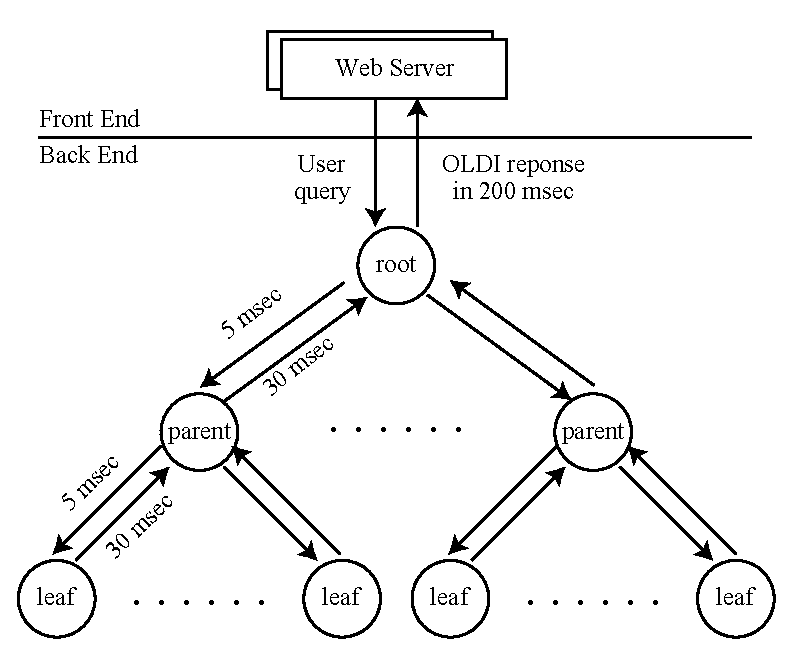
\includegraphics[autoebb, width=200pt]{./img/OLDI.pdf}
    \caption{OLDI architecture}
    %\ecaption{The control loop in DCTCP}
    \label{fig:oldi_tree}
    \end{center}
\end{figure}

\chapter{Motivated work}
\label{chapter:motivated_work}
この章では, 分散処理フレームワークを用いることで, フローサイズの小さい大量のQueryが発生し, MPTCPは,
フローサイズの小さいトラフィックに対しては, TCPよりも性能が劣化すると報告された問題~\cite{improving}に対して, 大規模データセンターネットワークへのMPTCP適用時の問題点を把握するために,
フローサイズの小さいトラフィックに対する性能を検証, ならびにクラウドサービスを想定したトラフィックの一例として並列分散処理アプリケーションを用いた二種類のトラフィックの測定結果を示す.
測定結果からトラフィックの特徴を示す事で, 従来のTCPで構成されたクラスターの抱えるボトルネックと複数のキュー,
複数の経路を持つマルチパス環境におけるデータセンターモデルの利点をそれぞれ示し, 提案手法の設計指針とする.

\section{評価実験と考察}
\label{sec:evaluation}
この章では, MPTCPデータセンターネットワークに対して実際のデータセンター環境を想定したシミュレーション実験を行い, その結果について考察する.

\subsection{想定環境}
今回, データセンター上でpartition-aggregateモデルに従う分散処理を想定する.
ネットワークトポロジーについては, 前章のFatTreeトポロジーを用い, 一つのPodが管理ノード群として他Podの12ノードに対し,
処理を指示することを想定する.
またベンチマークトラフィックについては, \ref{sec:traffic_scenario}節で述べた, 2つのトラフィックパターンについて評価・考察を行う.
メトリックとして表\ref{metric}を考える.
\begin{table}[t]
\begin{center}
\begin{tabular}{c|c}
\hline
トラフィックパターン & メトリック \\ \hline \hline
Query traffic & フロー完結時間[sec] \\
Short message traffic & フロー完結時間[sec] \\
\hline
\end{tabular}
\caption{トラフィックパターンごとのメトリック}
%\ecaption{Metric of each traffic patern}
\label{metric}
\end{center}
\end{table}

\subsection{シミュレーション結果}

\subsubsection{Query traffic}
Query trafficに対する評価として, フローサイズは1[KB]$\sim$16[KB]とした,
12の処理ノードへ平均200[ms]のポアソン生起でトラフィックを発生させ, フロー完結時間を測定した.
また, Query trafficのみ発生させた場合と, 50\%の処理ノードに対し継続的にデータを送信するトラフィックを, Background
trafficとして同時に発生させた場合の2パターンについて評価を行った.
その結果を, 図\ref{fig:pure_query}, \ref{fig:mix_query}に示す.
なお, エラーバーとして99\%信頼区間を採用した.

この結果から, MPTCPはQuery trafficに対し, 直接性能に影響を及ぼさず, Background
Trafficによる影響が性能差を生じさせたことが分かる.
これは, やはりMPTCPがTCPよりも帯域を大きく占有した影響を受けたと考えられる.
\begin{figure}[t]
 \begin{minipage}{0.5\hsize}
  \begin{center}
    \includegraphics[autoebb, width=120pt]{./img/pure_query.pdf}
    \caption{Query trafficフロー完結時間 (Background trafficなし)}
    %\ecaption{Flow completion time \newline of Query traffic
    %\newline with Background traffic}
    \label{fig:pure_query}
    \end{center}
 \end{minipage}
 \begin{minipage}{0.5\hsize}
  \begin{center}
    \includegraphics[autoebb, width=120pt]{./img/mix_query.pdf}
    \caption{Query trafficフロー完結時間(Background trafficあり)}
    %\ecaption{Flow completion time \newline of Query
    %traffic \newline with Background traffic}
    \label{fig:mix_query}
    \end{center}
 \end{minipage}
\end{figure}

\subsubsection{Short message traffic}
Short message trafficに対する評価として, フローサイズは50[KB]$\sim$1[MB]とした.
50\%の処理ノードに対し継続的にデータを送信するトラフィックを, Background trafficとして同時に発生させた状態で,
同時に12の処理ノードへ平均500[ms]のポアソン生起でトラフィックを発生させ, フロー完結時間を測定した.
その結果を, 図\ref{fig:short_query}に示す.

この結果から, MPTCPはShort message trafficに対し, フロー完結時間を短縮させたことが分かる.
これは, 先ほどのQuery trafficよりも大きなサイズのフローを流したので, MPTCPにより複数経路を利用し, TCPよりも短縮したことが考えられる.
実際, フローサイズが小さいと, MPTCPとTCP間でフロー完結時間の差が小さくなっている.

\begin{figure}[t]
    \begin{center}
    \includegraphics[autoebb, width=200pt]{./img/mix_short.pdf}
    \caption{Short message trafficフロー完結時間(Background trafficあり)}
    %\ecaption{Flow completion time  of Short message traffic with Background
    %traffic}
    \label{fig:short_query}
    \end{center}
\end{figure}


\subsubsection{Background traffic}
Background
trafficに対する評価として全12の処理ノードへ平均500[ms]のポアソン生起でフローサイズ1[KB]$\sim$1[MB]のトラフィックを同時に発生させた状態で,
同時に12の処理ノードへ平均500[ms]のポアソン生起でトラフィックを発生させ, 各経路のスループットを計測した.
その結果を図\ref{fig:background}に示す.

この結果から, MPTCPはBackground trafficに対し, TCPよりも性能向上が見られることが分かる.
これは, MPTCPのロードバランスと複数経路を使って並行的にデータを送信したことによるものである.

\begin{figure}[t]
    \begin{center}
    \includegraphics[autoebb, width=200pt]{./img/back.pdf}
    \caption{Background trafficスループット}
    %\ecaption{Throughput of background traffic}
    \label{fig:background}
    \end{center}
\end{figure}
\hspace{1cm}


\section{再現シミュレーション}
この節では, Raiciuらによって示したFatTree-MPTCPネットワークモデルでのフローサイズの小さいトラフィックに対する性能評価シミュレーションを再現し,
解析を行った結果を示す.

\subsection{再現シミュレーション実験環境}
Raiciuらは~\cite{improving}において, 各プロトコルがフローサイズの小さなトラフィックに対して及ぼす影響の評価を行い,
フローサイズの小さいトラフィックに関しては, MPTCPによりフロー完結時間を遅延させることを示した.
そのときのシミュレーション環境は, 以下の通りである.
ネットワークトポロジーには, 4:1にオーバーサブスクリプションされたFatTreeを用いている.
ベンチマークトラフィックについては, host-to-hostの1対1通信を用いている.
全てのhost-to-host通信のうち, 33\%をTCPまたはMPTCPにより継続してデータ転送 (Back-ground traffic)を行う.
残りのhostを使って, TCPによる70Kbyteのデータ転送をを毎200[ms]のポアソン生起させ, 転送完了までにがかかった時間を計測している.

今回の再現実験にはns-3 Direct Code Execution~\cite{ns3}を用い, MPTCPは, Linux
カーネルソースを用いた~\cite{mptcp_linux}.
図\ref{fig:fattree_rep}に, シミュレーションで用いたFatTree(k=2)トポロジーを示す.
このトロポロジーでの物理パスでは, 一つのサブフローが1本の物理パスを占有するように, 設計している.
すなわち, 4つのサブフローを使う場合, ホストには4本のインターフェースに対しそれぞれ4つIPアドレスが割り当てられる.
また, Host-Edge部分には, IPアドレスの数だけインターフェースを用意し, Aggregation-Edge部分も,
それに従いインターフェースを追加する.
さらにルーティングに関しては, Core1$\sim$Core4に分散するようにルーティングテーブルを設定した.

表\ref{table:testbed}に再現シミュレーション環境に対する各パラメータをまとめる.
\begin{table}[t]
\begin{center}
\begin{tabular}{c|c}
\hline
環境パラメータ & 値 \\ \hline \hline
ノード数 & 16 \\
MPTCP & v0.86 \\
帯域-core-aggr & 400Mbps \\
帯域-aggr-edge & 200Mbps \\
帯域-edge-host & 100Mbps \\
RTT & 0.5ms\\
バッファ & 100KB \\
\hline
\end{tabular}
\caption{ネットワークシミュレーション環境}
%\ecaption{Testbed on network simulation}
\label{table:testbed}
\end{center}
\end{table}

\begin{figure}[t]
    \begin{center}
    \includegraphics[autoebb, width=200pt]{./img/fattree_rep.pdf}
    \caption{再現シミュレーション環境でのネットワークトポロジー}
    %\ecaption{Network topology on reproducing simulation}
    \label{fig:fattree_rep}
    \end{center}
\end{figure}

\subsubsection{設定パラメータに対する有効性の検証}
伝搬遅延についてはRTT(Round Trip Time)として, 0.5[ms]に設定した.
これは, 一般的なデータセンター内のRTTが1[ms]以下であるためである~\cite{rtt}.

ウィンドウサイズについては, 以下の帯域幅遅延積(BDP)の式から, 400Mbpsを最大限利用できるだけの値を設定した.
\begin{eqnarray}
BDP[{\rm byte}] = 帯域幅[{\rm bps}] \times RTT \div 8
\label{cong}
\end{eqnarray}

各帯域については, 16のノードを使って輻輳を引き起こす現象を再現するために, 実際のデータセンターのような広帯域のネットワークと比べ,
狭い帯域を設定した.

\subsection{再現結果}
図\ref{fig:short_flow_rep}, 表\ref{table:short_flow_rep}に, 上記の実験環境で再現した結果を示す.
再現結果から, フローの様子を完結時間別に4パターンに分類することができることが分かった.
表\ref{table:flow_pattern}にそのフローパターンの定義を示す.

\begin{figure}[t]
    \begin{center}
    \includegraphics[autoebb, width=245pt]{./img/flow_comp.pdf}
    \caption{再現実験結果}
    %\ecaption{The result of the reproduction experiment}
    \label{fig:short_flow_rep}
    \end{center}
\end{figure}

\begin{table}[t]
\begin{center}
\begin{tabular}{c|p{6em}|c|p{6em}}
\hline
プロトコル & 平均フロー完結時間[ms] & 標準偏差[ms] &
95パーセンタイル[ms] \\
\hline \hline TCP &\hfil 78.4 & 122.5 &\hfil 266.7\\
MPTCP &\hfil 91 & 140.6 &\hfil 510.5\\
\hline
\end{tabular}
\caption{再現実験-平均フロー完結時間, 標準偏差}
%\ecaption{Average flow completion time and stdev on reproduction experiment}
\label{table:short_flow_rep}
\end{center}
\end{table}

\begin{table}[t]
\begin{center}
\begin{tabular}{c|c|c}
\hline
フローパターン & 完結時間[ms] & パケットロスの有無 \\ \hline \hline
Full window & $\sim$30 & なし\\
Intensive flow & $\sim$60 & なし\\
Delay with loss & 200$\sim$300 & あり\\
Extreme delay & 300$\sim$ & あり\\
\hline
\end{tabular}
\caption{完結時間別のフローパターン}
%\ecaption{Flow pattern classified by completion time}
\label{table:flow_pattern}
\end{center}
\end{table}


\subsection{考察}
表\ref{table:flow_pattern}に示した各フローパターンについて, それぞれの特性を分析する.

\subsubsection{パケットロスが発生しないフローパターン}
図\ref{fig:full_intensive}にFull windowとIntensive flowのデータ転送の様子を示す.

Full windowでは, TCPコネクション確立後, サーバーがすぐに最大ウィンドウサイズ分だけパケットを送り,
クライアントからのACKが返ってくると, 随時次のパケットを送っていた.
これは, 経路に輻輳がなく, 多くのウィンドウを利用できたということであり, 30[ms]以下でデータ転送を完了した.

一方, Intensive flowでは, サーバーが最大ウィンドウサイズ分に満たない量のパケットを送り,
クライアントからまとめて送られてくるACKを受け取った後, 集約してパケットを送っていた.
その結果, コネクションの切断時に, Full windowと比較して遅延を引き起こし60[ms]程度転送時間がかかった.

\subsubsection{パケットロスが生じたフローパターン}
図\ref{fig:delay_loss}にDelay with lossとExtreme delayのデータ転送の様子を示す.
いずれのフローパターンもデータ転送中にパケットロスが発生し, 再送処理, 重複ACK確認応答を行った.
パケットロスが起きた原因は, 短時間にフローサイズの小さいトラフィックが中継ルータを集中したためである.
実際, 200[ms]のポアソン生起のうち, 数10ms単位の短い期間でトラフィックが発生したとき, 中継ルータにおいてパケットロスが生じた.

Delay with lossでは, TCPコネクション確立後に数パケットのデータ転送を行い, パケットロスによるタイムアウトを生じた.
その後, 再送処理を経て, Maximum Segment Size (MSS)である1460[byte]でパケットを伝送した.

一方, Extreme delayでは, TCPコネクション確立直後にパケットロスによるタイムアウトを生じた.
その後も, パケットロスは生じないものの, 400[ms]頃まで伝搬遅延が生じていた.
また, 図\ref{fig:delay_loss}における二つのグラフの傾きは, セグメントサイズ最小値の586[byte]に設定され,
転送速度が上がらなかったことを表している.
これは, 中継するルータにおいてQoE制御による帯域制限が発生したことを示している.
実際, 同時刻に流れていたBackground trafficのスループットには変化がなく, QoE制御のrate controlによりBack-ground
trafficのデータ転送が優先され, ベンチマークトラフィックにはウィンドウサイズが制限されたと考えられる.

\begin{figure}[t]
 \begin{minipage}{0.5\hsize}
    \begin{center}
    \includegraphics[autoebb, width=120pt]{./img/full_intensive.pdf}
    \caption{Full windowとIntensive flowの比較}
    %\ecaption{\parbox{10em}{Comparison between Full \newline window and
    %Intensive flow}}
    \label{fig:full_intensive}
    \end{center}
 \end{minipage}
 \begin{minipage}{0.5\hsize}
    \begin{center}
    \includegraphics[autoebb, width=120pt]{./img/loss.pdf}
    \caption{Delay with lossとExtreme delayの比較}
    %\ecaption{\parbox{10em}{Comparison between Delay with loss and
   % Extreme delay}}
    \label{fig:delay_loss}
    \end{center}
 \end{minipage}
\end{figure}

\subsubsection{TCP v.s. MPTCP}
今回の再現実験において, TCPとMPTCPでフロー完結時間に差を生じた要因は, パケットロスが発生する割合にある.
図\ref{fig:cdf}に再現実験でのフロー完結時間ごとの累積確率分布を示す.
パケットロスを生じないフローに関しては, 両者に性能差を感じなかったが, この図から, MPTCPを用いた方が,
パケットロスを引き起こし遅延を生じさせる割合が大きいということが分かる.

このようにMPTCPが帯域を大きく占有することにより他のトラフィックを圧迫することは, MPTCPの輻輳制御によるものだと考えられる.
混雑のない経路でデータ転送する場合, MPTCPでは積極的にウィンドウサイズを増やそうとするため, 他のフローに対し遅延を引き起こしたと推測される.


\begin{figure}[t]
    \begin{center}
    \includegraphics[autoebb, width=200pt]{./img/cdf_rep.pdf}
    \caption{再現実験でのフロー完結時間の累積確率分布}
    %\ecaption{CDF of flow completion time on reproduction experiment}
    \label{fig:cdf}
    \end{center}
\end{figure}





\section{実トラフィック解析}

この節では, クラウドサービスを想定したトラフィックの一例として並列分散処理アプリケーションを用いた二種類のトラフィックの測定結果を示す.
測定結果からトラフィックの特徴を示す事で, 従来のTCPで構成されたクラスターの抱えるボトルネックと複数のキュー,
複数の経路を持つマルチパス環境におけるデータセンターモデルの利点をそれぞれ示し, 提案手法の設計指針とする.

測定環境には, 管理ノード1台(Master), 処理ノード10台の計11台のクラスターPCを用いた.
管理ノードは10GbpsイーサネットリンクでTop of Rack(ToR)スイッチに接続されている.

このクラスターPCでPresto~\cite{presto}によりインタラクティブなレスポンスを返す, 分散SQLデータベースを実現しており,
\S \ref{sec:traffic_scenario}で示した三種類のトラフィックが混在している.
トラフィックの測定には, 管理ノードのインターフェースを用いて, tcpdump\cite{tcpdump}によるパケットレベルの測定を行った.

{\bf 定常状態: }
管理ノードに対し, ジョブ命令を一切与えていない中で約10時間程度トラフィックを測定した.
図\ref{fig:constant}に定常時のフローサイズの累積分布を示す.
この分布から, 80\%以上のフローが10KB以下であるようにショートフローの数が全体のトラフィックの大部分を占めていることがわかる.
一方で通信量に着目すると, フロー数は比較的少ないがフローサイズの大きいトラフィックが大半を占めている.

次に, 図\ref{fig:constant_cdf}に管理ノードへのトラフィックの影響を示す.
この分布が示すように, 各処理ノードから管理ノードへのトラフィックの割合が大きく, それぞれフローサイズも大きい.
一方で, 管理ノードから各処理ノードへのトラフィックについては, 比較的フローサイズの小さいトラフィックの割合が大きい.

さらに, 図\ref{fig:constant_conc}に時間毎の同時接続数の分布を示す.
図\ref{fig:constant_conc}中の長時間通信は通信時間が全測定時間の90\%以上であるフロー数を表している.
この分布が示すように, 各処理ノードから管理ノードへのトラフィックの同時接続数が多く, 積極的に通信が行われている.
また, 短い通信時間でスパイク性のある中で, 長時間通信を行うフローが固定的に存在している.
\begin{figure}[t]
    \begin{center}
    \includegraphics[autoebb, width=200pt]{./img/constant.pdf}
    \caption{Prestoクラスタの定常時のトラフィック分布}
    \label{fig:constant}
    \end{center}
\end{figure}

\begin{figure}[t]
    \begin{center}
    \includegraphics[autoebb, width=200pt]{./img/constant_cdf.pdf}
    \caption{管理ノードから見た定常時のトラフィック累積分布}
    \label{fig:constant_cdf}
    \end{center}
\end{figure}

\begin{figure}[t]
    \begin{center}
    \includegraphics[autoebb, width=200pt]{./img/constant_conc.pdf}
    \caption{定常時トラフィック:同時接続数の分布}
    \label{fig:constant_conc}
    \end{center}
\end{figure}

{\bf 並列分散処理実行時: }
管理ノードに対し, 約1分間程度で完了するSQLジョブを与えた中でジョブが完遂するまでの間トラフィック測定を行った.
SQLジョブには, ``$select * from \, \$テーブル where \, \$条件$"を実行し,
全ての処理ノードにジョブを与えられるようにした.
図\ref{fig:job}にジョブ実行時のフローサイズの累積分布を示す.
この分布が示すように, ショートフローの数が全体のトラフィックの大半を占めるが, 定常状態と比べると,
全体的にフローサイズ大きいトラフィックが増えている.
実際, 80\%以上のフローが110KB以下であるように, ショートフローの割合が小さくなった.
同様に通信量に着目すると, フロー数は比較的少ないがフローサイズの大きいトラフィックが大半を占めるという事が分かる.

次に, 図\ref{fig:job_cdf}に管理ノードへのトラフィックの影響を示す.
この分布が示すように, 各処理ノードから管理ノードへのトラフィックの割合が大きく, フローサイズは小さいものが多いことが分かる.
しかし, 図\ref{fig:constant_cdf}の定常時のトラフィックと比べると,
管理ノードから各処理ノードへのトラフィックの割合が大きくなっている.

さらに, 図\ref{fig:job_conc}に時間毎の同時接続数の分布を示す.
この分布が示すように, ジョブ実行中は全体的にフローの数は増え, とりわけ管理ノードから各処理ノードへのトラフィックの割合が大きくなっている.
さらに, ジョブ終了後も同時接続数が大きく変化していないことから, 長時間通信を行うフローが固定的に存在している.
また, 各処理ノードから管理ノードへのトラフィックに着目すると, ジョブ開始時に接続数が大きく増えている事から, バースト性があるトラフィックであるといえる.

\begin{figure}[t]
    \begin{center}
    \includegraphics[autoebb, width=200pt]{./img/job.pdf}
    \caption{Prestoクラスタのジョブ実行時のトラフィック分布}
    \label{fig:job}
    \end{center}
\end{figure}

\begin{figure}[t]
    \begin{center}
    \includegraphics[autoebb, width=200pt]{./img/job_cdf.pdf}
    \caption{管理ノードから見たジョブ実行時のトラフィック累積分布}
    \label{fig:job_cdf}
    \end{center}
\end{figure}

\begin{figure}[t]
    \begin{center}
    \includegraphics[autoebb, width=200pt]{./img/job_conc.pdf}
    \caption{ジョブ実行時トラフィック:同時接続数の分布}
    \label{fig:job_conc}
    \end{center}
\end{figure}

これらの分布から, クラウド型サービスを想定したトラフィックの特徴として以下の事が述べられる.
\begin{itemize}
  \item 定常時もジョブ実行時も同様に, 管理ノードへ送信されるトラフィック量は多い
  \item 長い時間通信を行うフローが固定的に存在している
  \item ジョブ実行時の処理ノードから管理ノードへのトラフィックには, フローサイズも小さく, バースト性がある
\end{itemize}

また, これらの特徴から, 管理ノードへのトラフィックの集中, ショートフローのバースト性,
そして長時間通信を行うBackgroung trafficの問題が生じていると考えられる.
従って, 管理ノードに対するトラフィックとして大きく二つのパターンを検討する必要がある.
\begin{enumerate}
  \item ジョブ開始時のバースト性のあるショートフロートラフィック
  \item アプリケーション性能に直接影響しないBackgroung trafficが通信している中で,
  低レイテンシ通信が求められているショートフローの通信
\end{enumerate}

こうしたトラフィックは主に, 複数の処理ノードから単一の管理ノードへの通信で発生する.
そして, 中継スイッチ, エンドノードともに単一のNICキューへとトラフィックが集中する事で, ボトルネックになり,
ショートフローの遅延が問題となる\cite{bottleneck}.

\subsection{性能障害}
\label{sec:expected_effect}
次に, これらのトラフィックパターンが引き起こす可能性のある二ヶ所のボトルネックについて検討する.

\subsubsection{スイッチ - 性能障害}
現在のスイッチ機器では複数のフローを多重に扱うための共有メモリを持ち, 共有メモリプールからMMU(Memory Management
Unit)によって各インターフェースが利用できるメモリ量を動的に割り当てる事で, 複数の通信を公平に処理する事を目指す~\cite{flexible}.
しかし, 比較的安価なスイッチでは制御できるメモリ量が制限されているため,
様々な性能障害を引き起こす~\cite{flexible}.

{\bf Incast}\\
\label{subsec:incast}
図\ref{fig:impair}(a)に示すように, 短期間に一つのインターフェースへとフローが集中した場合, 用意されているキューが溢れ,
最悪の場合パケットロスを引き起こす.
こうしたトラフィックは, \S \ref{sec:traffic_scenario}で示したpartition-aggregate構造によるもので,
リクエストを受けた処理ノードが同期して一斉にレスポンスを返すことにより,
そのレスポンスを集約して受け取るノードが接続しているスイッチでのインターフェースのキューサイズが大きくなり, 遅延, パケットロスを生じる.
% こうした問題に対して, アプリケーションレベルにおいては二つのアプローチがある.
% 一つは, レスポンスのサイズを意図的に小さくし, スイッチバッファの圧迫を抑えることである.
% もう一つは, それぞれのリクエストにジッタを混ぜる事で, レスポンスを同期させないことである~\cite{synchro}.
% さらに, パケットロスを生じた際へのアプローチとしては, $RTO_{min}$を小さくする事でパケットロスの影響を抑える事ができる.

{\bf Queue buildup}\\
\label{subsec:queue}
\S \ref{sec:traffic_scenario}で示したように, 並列分散処理のレスポンスには直接影響しないBackgroung trafficは,
スイッチバッファにパケットロスを引き起こすほどの影響を及ぼし, そのインターフェースがボトルネックとなる可能性がある.
図\ref{fig:impair}(b)に示すように, Backgroung trafficとQuery trafficが同じインターフェースを利用する場合に,
サイズの大きいフローによるショートフローのキューイング遅延が生じる.
このとき, Query trafficには{\it Incast}とは異なり, バースト性は必要ではない.
% このキューイング遅延の問題に対する解決策は, キューに溜まったパケットを素早く排出することで, キューサイズをなるべく小さく保つことである.

\begin{figure}[t]
    \begin{center}
    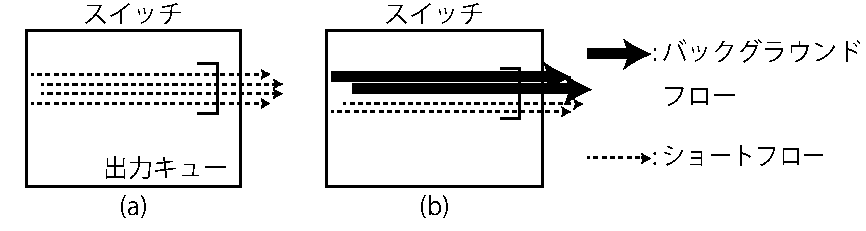
\includegraphics[autoebb, width=200pt]{./img/impairments.pdf}
    \caption{中継スイッチで引き起こすボトルネック}
    \label{fig:impair}
    \end{center}
\end{figure}


\subsubsection{エンドノード - 性能障害}
今日のGbE(Gigabit Ethernet)通信において, 割込み処理は大きなボトルネック要因の一つである.
例えば, 1GbEにおいて64バイトフレームの最大受信可能数は, 毎秒約150万であり, 1パケット受信する度に割り込み処理を行うと,
CPUリソースが枯渇する.
そのため, 割込み処理の回数を抑えることが必要であるが, その分レイテンシが上がる可能性があり, 互いのトレードオフを適切に対処し高い性能を得る必要がある.
また, 今日の多くのCPUはマルチコアであり, CPUリソースを効率的に利用する事が求められている.

{\bf 割込み処理}\\
パケット受信の際のNICによるハードウェア割込みは, 即座に受信処理を行う事ができ, キューイングの遅延を小さくする事ができる.
しかし, 割込み処理が増えれば, その分オーバヘッドが大きくなり, OSの性能が劣化する.
割込み処理を扱う代表的な仕組みとして, ポーリング, interrupt coalescingがある.

ポーリングはNICの割り込みを使わず, タイマーにより定期的にNICの受信キューを監視することで, 割り込み負荷を軽減するソフトウェア技術である.
しかし, NICでパケットを受けてから即座に処理できない為, 遅延が発生する場合がある.
現在のLinuxカーネルにおいては, NAPIにより, 通信量が多く高負荷時にはポーリングが作用する~\cite{NAPI}

interrupt coalescingは, 複数のパケット, あるいは一定期間待ってからをまとめて一度で割り込ませる事で,
割込み回数を減らすハードウェア技術である.
しかし, ポーリングと同様, 即座に処理できない為, 遅延が発生する場合がある.

{\bf プロトコル処理}\\
マルチコア環境においても基本的には一つのNICの受信処理は1つのCPUでしか行えない.
そのため, ハードウェアへのアプローチとして, 1つのNICに複数の受信キューを持たせて, 受信処理をそれぞれのCPUへ分散させている, Receive
Side Scaling(RSS)がある~\cite{RSS}.
しかし, 一般に複数受信キューを持ち, RSS機能があるNICは高価である\cite{intel}.
そのため, 一つしか受信キューを持たないNICであっても, 複数のCPUを分散させるソフトウェア技術として, RPS(Receive Packet
Sterring)がある~\cite{RPS}.
% しかしRPSでは, プロトコル処理とアプリケーション処理のCPUが異なる場合が生じ, その問題を最適化したのがRFS(Receive Flow
% Sterring)がある~\cite{RFS}.
これらの技術により, CPUの複数のコアをより効率良く利用する事ができる.
また, プロトコル処理やアプリケーションでの処理については, RPS等で複数のCPUへと分散させる事ができるが,
その際の割込み処理についてはオーバヘッドが生じる可能性がある.


\section{検証実験}
\label{sec:verification}
% これまでの研究において報告されたMPTCPによるショートフロー性能劣化の問題~\cite{improving}を受け, その再現実験を行うことにより,
% 原因を解析し, 二つの要因を明らかにした~\cite{mptcp_ana}.
% 一つ目は, MPTCPはTCPよりも多くのトラフィックを排出し, より多くのNICインタフェースを利用する事で,
% 中継スイッチにおいてショートフローが利用するインタフェースと競合し, スイッチでの遅延, パケットロスが生じるということ.
% 二つ目は, ショートフロートラフィックのバースト性の問題により, エンドノードで単一のNICに負荷が集中し, 受信処理の遅延が生じたということ.
% これらの結果を受け,
% 低レイテンシでの通信が求められるショートフローに対して, MPTCPによるバックグラウンドトラフィックが利用しているインタフェースを回避し,
% 比較的輻輳が起こっていない経路を適切に選ぶ事で,
% 単一キューへの通信負荷の問題は解消され, ショートフローのフロー完結時間(FCT)が改善できるのではないかと, 仮説を立てた.
この章では, 実機での実験を用いて, 低レイテンシでの通信が求められるショートフローに対して, バックグラウンドトラフィックが利用しているインタフェースを回避し,
適切に経路を選ぶ事で, 単一キューへの通信負荷の問題は解消され,
ショートフローのフロー完結時間(FCT)が改善できるという仮説の検証, また複数のキュー,
複数の経路を利用した経路切り替えによる改善手法に対する予備実験を行う.
具体的には, 中継スイッチとエンドノードへのそれぞれの単一キューの負荷について, 複数のNICを用いて分散させ, その効果を検証する.

\subsection{実験環境}
{\bf (1)中継スイッチに対する負荷実験}\\
ネットワークトポロジーには, 2段で構成されたトポロジーを用いる.
図\ref{fig:topology_switch}に, 用いたトポロジーを示す.
ベンチマークトラフィックについては, 二つのペアに対してエンドノード同士の1対1通信を用いている.
一方のペアに対しては, シミュレーションを実行している間, 継続してデータ転送 (バックグラウンドトラフィック)を行う.
他方のペアに対しては, TCPによる70Kbyteのデータ転送(ショートフロー)を毎10ms一様生起させ,
転送完了までにかかった時間FCT(Flow Completion Time)を計測する.
ショートフローのルーティングに関しては,
図\ref{fig:topology_switch}に示す3つのパターンを用いて中継スイッチへのキューイング負荷の影響を検証する.


{\bf (2)エンドノードに対する負荷実験}\\
ネットワークトポロジーには, 二つのNICを持った二つエンドノード同士をL2スイッチを介してそれぞれのNIC毎に接続した.
図\ref{fig:topology_node}に, 用いたトポロジーを示す.
ルーティングに関しては, それぞれの対をなすNIC同士が通信を行う.
ベンチマークトラフィックについては, エンドノード同士の1対1通信を用い, ショートフローとバックグラウンドフローを通信させる.
バックグラウンドフローについては,
ショートフローが通信しているNICペアと同じものを使って共有して通信させるパターンとショートフローが通信しているNICペアとは異なるペアのNICを用いて通信を行うパターンの2パターンについて検証する.
ショートフローは, TCPによる70Kbyteのデータ転送を毎10ms一様生起させ, 転送完了までにがかかった時間を計測している.
バックグラウンドトラフィックは, シミュレーションを実行している間, 継続してデータ転送を行う.

表\ref{table:experiment_ver}に用いた機器の詳細を示す.
\begin{figure}[t]
    \begin{center}
    \includegraphics[autoebb, width=200pt]{./img/topology_ns3.pdf}
    \caption{中継スイッチへのNIC負荷実機実験トポロジー}
    \label{fig:topology_switch}
    \end{center}
\end{figure}

\begin{figure}[t]
    \begin{center}
    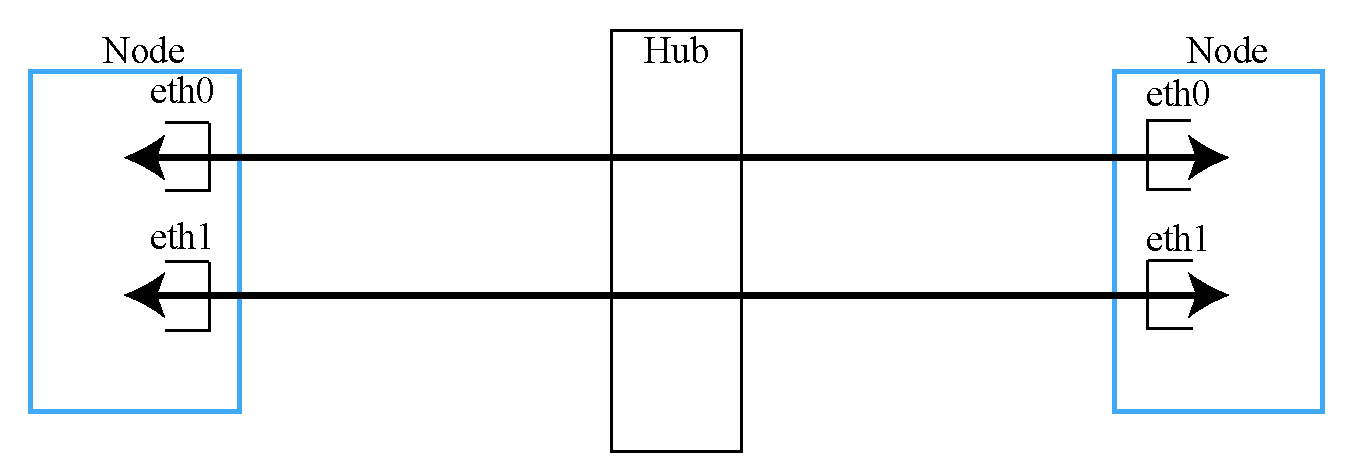
\includegraphics[autoebb, width=200pt]{./img/topology_real.pdf}
    \caption{エンドノードへのNIC負荷実機実験トポロジー}
    \label{fig:topology_node}
    \end{center}
\end{figure}

\begin{table}[t]
\begin{center}
\footnotesize
\begin{tabular}{c|c}
\hline
項目 & スペック \\ \hline \hline
OS & Linux 3.13.0 \\
CPU & Intel Xeon CPU L3426 \\
メモリー & 4GByte \\
NIC対応ドライバ & e1000 \\
スイッチ-実験1 & Catalyst 2940(100T) \\
スイッチ-実験2 & GS905L V2(1000T) \\
リンク & 1GbE \\
\hline
\end{tabular}
\caption{実験環境パラメータ}
\label{table:experiment_ver}
\end{center}
\end{table}

\subsection{実験結果}
{\bf (1)中継スイッチに対する負荷実験}\\
図\ref{fig:improve}に上記の実験環境での結果として, 70KBのショートフローのFCTとバックグラウンドフローの経路利用率を示す.
FCTの箱ひげ図の上端には, 95パーセンタイル値, 下端には最小値を用いている.
最大値でなく95パーセンタイル値を採用したのは, 特に遅延した下位5パーセントに着目することで, 遅延した割合の大きさを比較するためである.
このメトリックにより, コンスタントにアプリケーション性能の出せるデータセンターネットワークの実現への指針となる.
この結果から, ショートフローの通信が中継スイッチにおいて, バックグラウンドフローと経路およびインターフェースを共有した影響で,
一部のフローが大きく遅延し, その分散が大きくなっている事が分かる.
一方で, 同じスイッチでインタフェースは共有しなかったフローに対しては大きな影響はなかった.
これは, 単一NICキューに対して二つのトラフィックが集中したことによる遅延の影響であると考えられる.
その影響からバックグラウンドフローに対しても, スループットが下がっている事が分かる.

これらの事から, アプリケーション性能に直接影響しないバックグラウンドフローが通信している中で,
低レイテンシ通信が求められているショートフローの通信をする際, 中継スイッチでの利用するインタフェースが競合する場合,
単一のキューに対しトラフィックが集中し, 受信処理の割込みのオーバヘッドや, プロトコル処理の遅延の影響が生じたと考えられる.

\begin{figure}[t]
    \begin{center}
    \includegraphics[autoebb, width=200pt]{./img/switch_verif.pdf}
    \caption{中継スイッチに対する負荷実験での70kbベンチマークトラフィックに対するフロー完結時間とリンク利用率}
    \label{fig:improve}
    \end{center}
\end{figure}


{\bf (2)エンドノードに対する負荷実験}\\
図\ref{fig:real_exp0}に上記の実験環境での結果として,
70KBのショートフローのFCTとそれぞれの経路の利用率を示す.
FCTの箱ひげ図の上端には, 95パーセンタイル値, 下端には最小値を用いている.
この結果から, ショートフローの通信が, エンドノード間通信において, バックグラウンドフローと経路およびインターフェースを共有した影響で,
FCTの分散が大きくなっている事が分かる.
一方で, 経路, インタフェースは競合しなかったものの, バックグラウンドフローとショートフローが同時に通信を行ったことで若干の遅延の影響が生じ,
分散が大きくなっている.
これは, 単一NICに対して二つのトラフィックが集中したことによる負荷分散の効果が得られたが, プロトコル処理以降の部分で,
複数のフローが同時に通信を行った事に対するオーバヘッドが生じたと考えられる.
またバックグラウンドフローに着目すると, インターフェースを共有した場合においては,
ショートフローだけでなくバックグラウンドフローにも遅延が生じ, スループットが低下している.

これらの事から, アプリケーション性能に直接影響しないバックグラウンドフローが通信している中で,
バースト性のあるショートフロートラフィックの通信をする際, エンドノードに対して, 利用するインタフェースが競合する場合,
単一のNICに対しトラフィックが集中する事で, 受信処理の割込みのオーバヘッドや, プロトコル処理の遅延の影響があると考えられる.


\begin{figure}[t]
    \begin{center}
    \includegraphics[autoebb, width=200pt]{./img/real_eth0.pdf}
    \caption{エンドノードに対する負荷実験での70kbベンチマークトラフィックに対するフロー完結時間とリンク利用率}
    \label{fig:real_exp0}
    \end{center}
\end{figure}

\subsection{考察}
\label{sec:analysis}
これらの解析結果から, エンドノード, スイッチに対する機能障害が引き起こる要因について述べ, 今後の改善手法の検討を行う.
大量の計算機資源をいかに効率的に利用するか, という課題を今日のデータセンターは抱えており,
並列分散処理アプリケーションを用いる事が一般的である.
今の並列分散処理システムがpartition-aggrigation構造である限り, 管理ノードや多段のクラスター構成であればアグリゲーターノードに対して,
処理ノードからのトラフィックが集中する問題は発生する.
その結果, Queue buildupやIncastのような単一キューへの負荷集中の問題が中継スイッチやエンドノードに対して生じ,
CPU性能を効率的に引き出せず, 並列分散処理の性能が劣化する.

こうした遅延の影響を軽減する為には, 混雑時の通信量を抑える制御を行う, あるいは混雑時にも空いているリソースを効率良く利用する事が必要である.
MPTCPによる既存の計算機資源に対して複数NICを用いて性能向上を目指すように,
複数のフローを通信する際に異なる物理インターフェースを利用する事で, マルチコアを持つCPUの効率的な利用につなげられる.
すなわち, 複数のキューに対して通信を分散させるようなトラフィック制御により,
例えばレイテンシ志向なショートフローとスループット志向なバックグラウンドフローのような役割の異なるトラフィックを共存させ,
最適な通信の実現が可能であることが実験により明らかとなった.
そのような物理的に複数のNICによりマルチキューが介在する汎用的な機器で構成されているネットワークの中で,
トラフィックをどのように制御するかという点については, スイッチやエンドノードのOSスタック等のどこで制御をするか, またどのようなアルゴリズムでそれを実現するかを検討する必要がある.

\subsection{Directing result}
\label{sec:analysis}
経路混雑時のトラフィック制御について, 今後の指針となる一つの結果を示す.
提案手法では, 適切な経路を選んで通信を開始をする必要がある.
経路を決める際のメトリックとしては様々なものが考えられ, その中の一つとして経路の利用率がある.
経路利用率がショートフローの通信に対してどのような影響があるのか示した結果を図\ref{fig:load_test}に示す.
実験環境には, 中継スイッチに対する負荷実験と同様であり, バックグラウンドフローの負荷の度合いを変化させた.
この結果から, 70 $\sim$ 80 $ \% $ の経路利用率の場合, 遅延するショートフロー発生する事が分かり,
適切な経路選択には利用率も一要因として考慮する必要がある.

\begin{figure}[t]
    \begin{center}
    \includegraphics[autoebb, width=200pt]{./img/load_test.pdf}
    \caption{スイッチに対する負荷実験でのバックグラウンドフローの影響}
    \label{fig:load_test}
    \end{center}
\end{figure}


\chapter{提案手法}
\label{chapter:proposal}
低レイテンシなデータセンターの研究動向と, 並列分散処理アプリケーションが生成する特有のトラフィックパターンが引き起こす機能障害をふまえて,
改善手法を提案する.
本提案手法では, 
汎用的なネットワーク機器で構成されたマルチパスなデータセンターネットワークにおいて, エンドノードのみの改良によって, 
長時間継続的にデータを転送し続けるトラフィックが通信している中でのサイズ小さいフロー通信に対する低遅延通信を達成することを目指す.
この目的を達成するために, 提案手法では指向が異なるフローを区別する制御を行うことで, レイテンシ指向なフローについてキューイング遅延を小さくする通信を行う.

\section{Motivation}
提案手法の動機となったのは, MPTCPを用いたデータセンターネットワークモデルである\cite{improving}.
今日のデータセンターネットワークは, FatTreeトポロジーやClosトポロジーに基づいた構成になっており\cite{dctcp, vl2},
等コストな経路が複数存在している. 
提案されたネットワークモデルでは, エンドノードが複数のNICを持ち,
MPTCPによって一つのフローの通信で複数の経路を同時に利用することでスループットを向上させる.
このような複数経路の効率的利用には, IPベースのルーティングで実現しており, それぞれのエンドノードが持つIPアドレスのペアにより, 通信経路が決定する.
現在のMPTCPの実装では, TCPコネクション確立後に互いのIPアドレスを交換し,
新しいサブフローを形成する仕組みになっており, サイズの小さいフローの通信では, サブフローが形成されないまま通信が完結する問題がある. 
その結果, 一つの経路に通信が集中することとなり, で中継スイッチのキューが圧迫され, フローの遅延が大きくなる可能性がある. 
実際, $\S$\ref{reproduction_simulation}での解析でも,
このコネクション確立の際に遅延が生じることが分かっており\cite{mptcp_ana}, どの経路を利用するかによって, 通信性能が大きく変わる.

複数経路の有効活用の手法として, ECMPによるフロー単位でのルーティングがある. 
ECMPではパケットヘッダーの5タプルを用いたハッシュベースのルーティングやラウンドロビンによって, ランダムに経路を選択し, 負荷分散していく. 
この不完全なランダム性のために, ショートフローとロングフローが同一の経路に振り分けられることが起こり,
ショートフローはFCFS(First-Come-First-Serve)方式のキューシステムによって, キューイング遅延が発生する. 
今, Fig.\ref{fig:repflow_scenario}のようなネットワークシナリオを考える. 
このトポロジーは$k=4$ FatTreeトポロジーでのある1ポッド内での通信を示している. 
スイッチS1(S2)と接続されている二つのノードともう一方のノード間にはと二つの等しいコストの経路があり, H2からH4に対してS1-S3-S2の経路を通り,
ロングフローが通信している状況を考える. 
今, H1はH3に対してショートフロー通信を行おうとしたとき, ECMPによるランダムルーティングにより,
$0.5$の確率で同じ経路S1-S3-S2を選択してしまう. 
その結果, ロングフローによるキューイング遅延の影響を受ける. 
実際, $\S$\ref{sec:verification}に示すように実機を用いてこの同一経路を通る問題を検証したところ,
ロングフローをうまく負荷分散した時と同一の経路で通信した時の95パーセンタイル値FCTにおいて,
約10倍程度性能が劣化することが分かった\cite{mptcp_ana2}.

従って, {\bf ロングフローはS1-S3-S2の経路を通り, ショートフローはS1-S4-S2の経路を通るように分散させて通信すること}が,
マルチパス環境における複数経路の効率的な利用の理想的な状況である. 

\begin{figure}[t]
    \begin{center}
    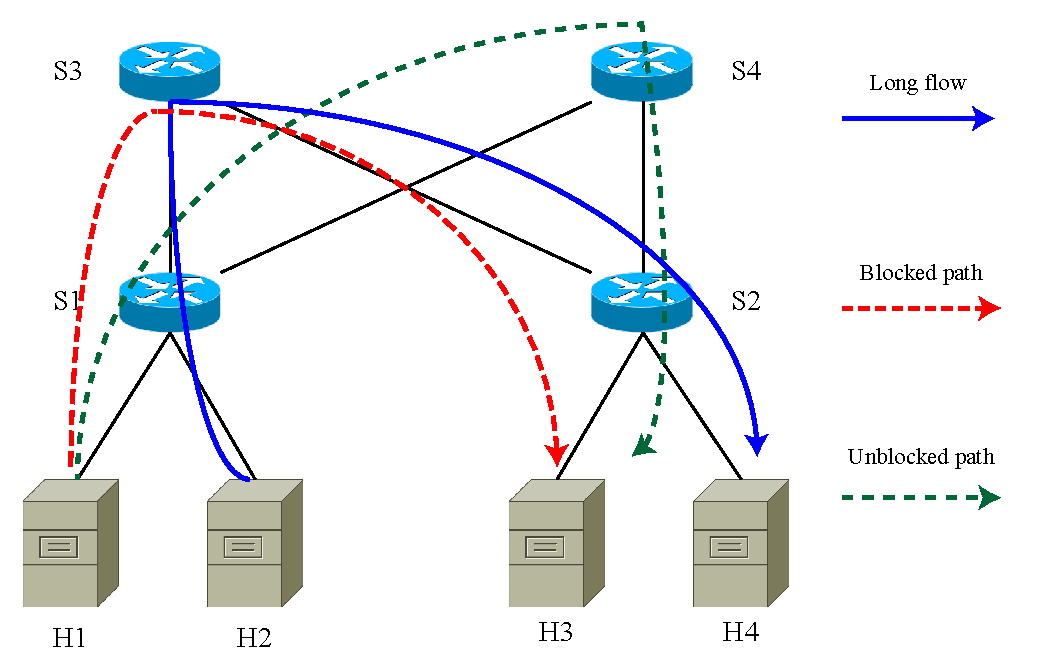
\includegraphics[autoebb, width=250pt]{./img/schenario.pdf}
    \caption{Scenario of queue buildup problem with multi-cost paths)}
    %\ecaption{The control loop in DCTCP}
    \label{fig:repflow_scenario}
    \end{center}
\end{figure}

$\S$\ref{chapter:related_work}に示した既存研究のように, 
データセンターネットワークでのショートフロー問題を解決するために多くの取り組みがされているが, 以下のような要求が考えられる. 
\begin{enumerate}
\item スイッチに対して特殊な実装を施さないこと. 
\item 既存のアプリケーションにも変更なく使えるようにすること. 
\item ショートフローのFCTだけでなく, ロングフローのスループットについても改善すること. 
\end{enumerate} 

1. については, $\S$\ref{chapter:related_work}に示した多くの手法がスイッチに対して変更を加え,
キューイング遅延が起こっている箇所から直接情報を得ることで, 改善を実現している. 
しかし, スイッチに対して変更を加えることで, 全てのスイッチに対してそれらを行う必要性があるため, 実環境への適用に問題があると言える. 
実際, 様々な種類のネットワーク機器が混在している中ではなおさら実現困難である\cite{d3}.

2. については, 既存研究の中でRepFlowは中継スイッチに変更を必要とせず, エンドノード間の変更のみで改善可能な手法であるが,
現状の実装だと, アプリケーションに対する変更が必要であるため, 既存のアプリケーションの変更が必要である\cite{repflow}.
そのため, 実現可能性の観点では有効であるとは言えない. 

3. については, $\S$\ref{sec:verification}に示すように, ロングフローとショートフローが同一の経路で通信を行った場合, 
ECMPによる負荷分散手法では深刻な遅延の問題を引き起こすこととなる. 
$\S$\ref{sec:verification}に示す検証実験では, ショートフローの性能劣化だけでなく,
ロングフローのスループットについても約30\%程度利用率が劣化する結果が得られた. 
RepFlowでは, ショートフローに対して同一の通信を複製することによって, キューイング遅延のない経路を通る,
ショートフローに対して最小のFCTを達成できるという手法であるが, 複製の結果, ロングフローのスループット性能も劣化することが考えられる. 

以上を踏まえて本研究における位置付けを以下のように設定する. 
\begin{enumerate}
\item エンドノード間のみのアプローチで改善を行う.  
\item OSのみに変更を加え, 既存のアプリケーションに変更を加えず適用できる. 
\item フローを指向ごとに区別し, それぞれに応じた改善を行うこと. 
\end{enumerate} 

今, Fig.\ref{fig:repflow_scenario}の環境において上記の前提の下, ロングフローとショートフローを区別し, 別々の経路を通るように分散させて通信することの実現を考える. 
しかし, 既存の技術では{\bf フローの区別}と{\bf それぞれの経路での通信}を達成することができない. 
フローの区別については, 基本的にはフローサイズの大きさで分類することができるが, OSから一つのフローを見た時に,
事前にどのくらいのデータが転送されるかを知る手段はない. 
たとえフローを区別できたとしても, それぞれのフローをどの経路に流すべきか判断するためのメトリックも既存のエンドノードでの技術にはない. 

そこで本研究では, あらかじめ通信経路を決定するために, データセンターネットワーク内に指向毎にレーンを設けるデータセンターレーンモデルと,
フローの指向を区別し, それぞれの経路を切り替えるためのアルゴリズムを提案する. 

\section{Design}
本節では, 本研究における位置付けの下で, 指向毎にフローを区別し, それぞれの経路に切り替えて通信を行うことを実現するため,
データセンターレーンモデルと経路状況を考慮した経路切替アルゴリズムを提案する. 

\subsection{データセンターレーンモデル}
\label{subsec:lane_model}
本小節では, 指向毎にフローを切り替えて制御するためのネットワークモデルとして, データセンターレーンモデルを示し,
そのトポロジーと動作するアーキテクチャについて示す. 

\subsubsection{背景}

今日のネットワーク機器はコモディティ化し, 安価な機器とある用途に特化した高価な機器のコストの差は明確となっており,
データセンター事業者はその性能とコストのトレードオフについて考慮しなければならず,
なるべくコストを抑えたい要求に対して頭を悩ませている\cite{fattree}.
50年以上前の電話網の形成の際にも, 多くの汎用的なスイッチを用いてより多くの端末に接続できるような設計が行われた\cite{clos}. 
そうしたClosトポロジーに基づき,
Ethernetスイッチによって構成されるネットワークトポロジーの一つにFatTreeトポロジーがある\cite{fattree}. 

Full-bisectionalなネットワークトポロジーに対する, 満たすべき要件として以下のようなものが考えられる\cite{improving}.
\begin{itemize}
\item 局所性のないトラフィック
\item すべてのホストが最大帯域活用できる
\item どのアクセスリンクに対してもトラフィックの集中がない
\end{itemize} 
%実際にはこれらの案件が同時に必要となる場合は起こり得ないと考えられ,
%Full-bisectionalな帯域を提供することはコストの面から最適であるとは言いにくい.

今FatTreeトポロジーに対して, 並列分散処理システムを適用させることを考え, Hadoop Distributed File
System(HDFS)によって同じラックの異なるホストにデータを複製し, MapReduceによるmapタスクがそれらに対して割り当てられるとする.
つまり, 同一ポッド内でのトラフィックが発生する.
MPTCPは基本的に複数の経路を持つ コア部分を経由するトラフィックに対して有効に働くが, このように経路選択肢が少ないローカルなトラフィックに対して,
十分に機能しない.

もしすべてのノードに対してMPTCPが実装されたとき, よりMPTCPの特性を引き出すようなトポロジーを検討する必要がある. 
具体的には, エンドノードとToR(Top-of-Rack)スイッチ間のアクセスリンクでボトルネックが発生した時, 効率的な帯域の利用を考える. 
手法として例えば, 1GEthernetリンクから10Gリンクへと変更することでより広帯域なネットワークを実現できるが, コスト面の問題がある. 
また, 従来のSigle-path TCPでは, 1本のリンク容量以上の帯域を得ることはできないという制限がある. 
しかしMPTCPでは, そのような制限はない. 
実際, 近年のサーバ機器には基本的に複数のギガビットイーサネットインタフェースが搭載されており,
エンドノードが二つのNICを持つ際のトポロジーのプロトタイプとして,
Fig.\ref{fig:dual-homing}のようなDHFT(Dual-Homing
FatTree)トポロジーが提案されている\cite{improving}.

\begin{figure}[t]
    \begin{center}
    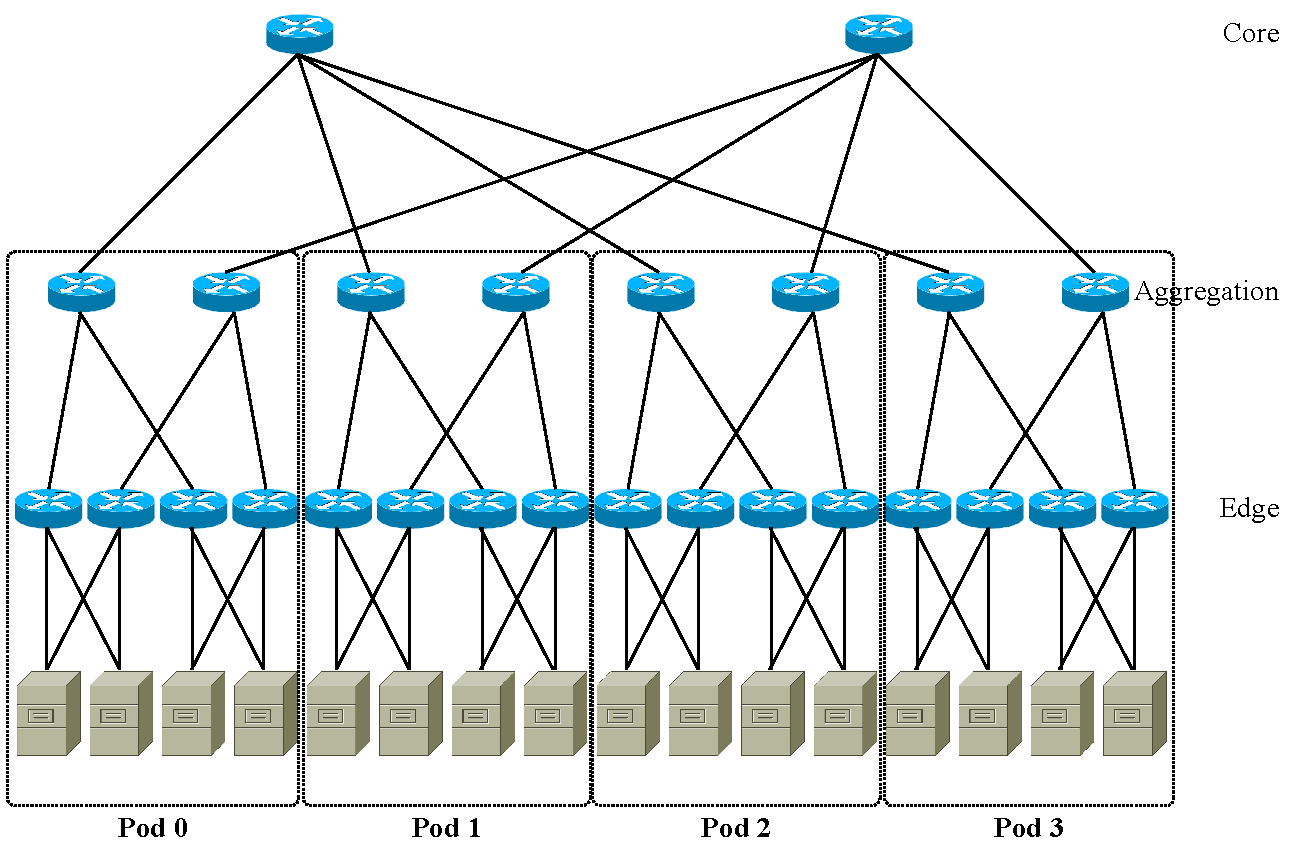
\includegraphics[autoebb, width=250pt]{./img/mhft.pdf}
    \caption{k=4 Dual-homing in the FatTree Topology}
    %\ecaption{The control loop in DCTCP}
    \label{fig:dual-homing}
    \end{center}
\end{figure}

\subsubsection{Motivation}

$\S$\ref{chapter:datacenter_network}にて示したように, 現在のMPTCPの実装では,
まず3ウェイ・ハンドシェイクによってTCPコネクションを確立し, その際にそれぞれの端末がMPTCPを利用可能かどうかのネゴシエーションを行う.
MPTCPが利用可能な場合, 互いの持っているIPアドレスを交換し(add\_address), その後サブフローを形成し, 複数の経路利用しながら通信を行う. 
その時MPTCPの輻輳制御によって, それぞれの通信状況に合わせてウィンドウサイズが調整され, 通信される\cite{balia}. 
しかし, 今のMPTCPではサイズの小さいフローについては, サブフローを形成する前に通信が完了する. 
そのため, たとえTCPコネクションを形成するための経路が混雑した状況であっても, MPTCPによってその経路を回避する手段はなく,
Fig.\ref{fig:repflow_scenario}で示したような性能劣化を導いてしまい,
マルチパス環境における複数経路の効率的な利用を実現できなくなる. 
ここで, 現状MPTCPを用いて経路選択をする上での課題を以下に示す. 
\begin{enumerate}
\item 基本的なIPベースのルーティングでは, コネクションを確立する経路は毎回同じである. 
\item あらかじめ経路を決定するには, 通信経路の輻輳状況を事前に把握しておく必要がある. 
\end{enumerate} 
1. についてはIPベースのルーティングでは基本的に宛先アドレスと送信元アドレスから決定されるので、コネクションを確立するアドレスペアが同じだと,
それに従い通信経路も同じものが選択される. 
異なる経路を選択するためには, 宛先アドレスとしてサーバ側の持つアドレスを事前に把握しておく必要があり,
その上でECMPやラウンドロビンのような分散手法の適用が考えられる.
しかし先に示したように, これらの分散手法では完全な負荷分散は実現できず, あらかじめ通信状況を取得するなどのアプローチが必要である. 

2. については, 本研究ではエンドノードに対する変更のみで改善を目指しているため, 遅延している中継スイッチから, 直接情報を得ることはできない. 
これまでの通信状況を把握しておくための取り組みとして, OpenFlowを用いた手法が提案されているが,
経路の統計情報を得るためのオーバーヘッドが発生するため, 現実的な解決策とは言えない\cite{devoflow}.

これらを踏まえて, 用途の異なるフローに対して通信経路を切り替えるため, データセンターレーンモデルを提案する.

\subsubsection{アーキテクチャ}
複数のインタフェースを持つエンドノードに対してFatTreeトポロジーを用いて, 指向毎のフローを切り替え制御の実現を目指す.  
具体的には複数の等価コストな経路に対してレーンを定義し, 区別したフローに対して通信を行う経路を設置する. 

このモデルの狙いは, スイッチから直接情報を得るような粒度の細かい制御を用いて遅延を回避するのではなく,
あらかじめ通信すべき経路を区別しておくことで, それぞれの目的にあった通信を実現することにある. 
データセンターレーンモデルでは, 以下のような用途のレーンが設置される. 
\begin{itemize}
\item {\it Query traffic}や{\it Short message
traffic}のようになるべく短いFCTで通信したいショートフロートラフィックに対しては, レイテンシ指向なフローとみなし,
常に空いている状態に保たれたショートフローレーンSL(Short-flow Lane)を用いる.
\item {\it Backgroung traffic}のようにより大きなスループットで通信したいロングフロートラフィックに対しては,
スループット指向なトラフィックとみなし, 一般に複数の経路が設置してあるロングフローレーンLF(Long-flow lane)を用いる. 
\end{itemize}

Fig.\ref{fig:lane_model}にネットワークレーンモデルを示す. 
今, 互いのエンドノードはそれぞれのインタフェースごとにIPアドレスを持っているとし, それぞれ$Lane Info$が与えられているとする. 
この$Lane Info$の値は, 各ノードのOSに対して設定するパラメータであり, 各ノードが保有している送信元アドレスと1対1に紐付いている. 
% このとき, 中継するスイッチでは各インターフェース毎に経路を分散されることが望ましい.  
これにより, 初めのTCPコネクションを形成する$src:10.1.0.1, dst:10.2.0.1$の通信に対しては, Path1でコネクションを形成し, 
次に, 互いのアドレス$(10.1.1.1, 10.2.1.1.)$を交換し, サブフローを形成できる状態にする. 
サブフロー$src:10.1.1.1, dst:10.2.1.1$の通信に対しては, Path2を利用される. 
このように, それぞれのサブフローの通信においては, 異なる経路を形成し, 通信が行われる. 
従って, 送信元アドレスが決定した時点で, 通信経路が決定するため, 送信元アドレスと紐付いている$Lane
Info$が通信経路のレーンを示していることになる.

\begin{figure}[t]
    \begin{center}
    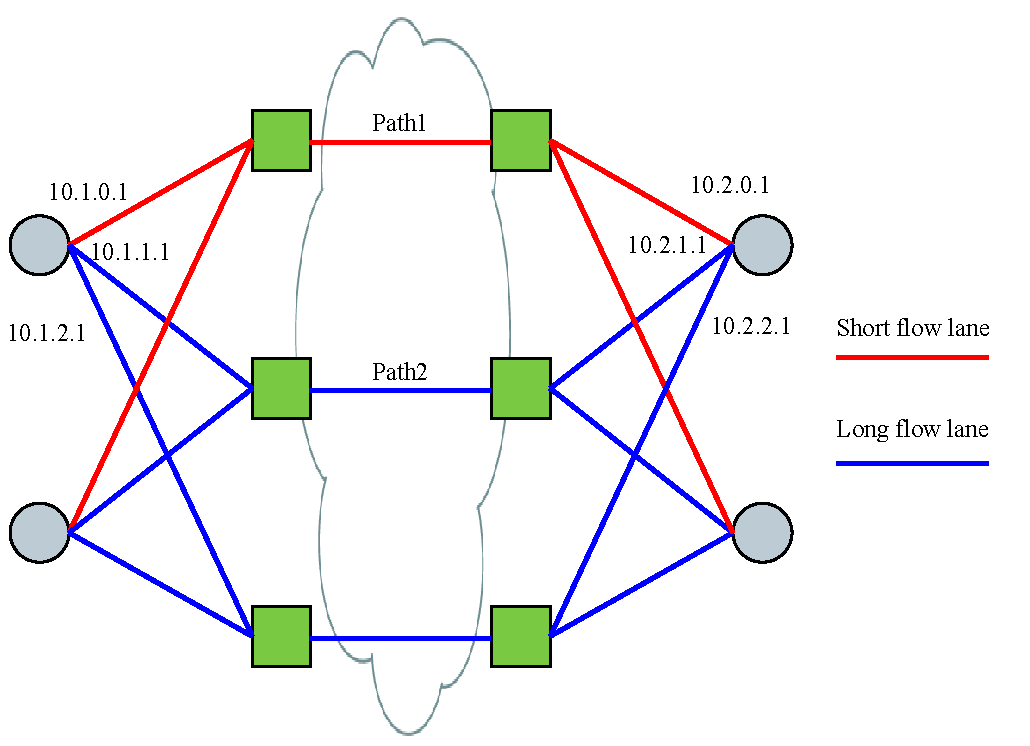
\includegraphics[autoebb, width=250pt]{./img/lane_model.pdf}
    \caption{Datacenter Lane Network Model}
    %\ecaption{The control loop in DCTCP}
    \label{fig:lane_model}
    \end{center}
\end{figure}

\subsection{経路切り替えアルゴリズム}
次に, $\S$\ref{subsec:lane_model}にて示した, データセンターレーンモデルに対して, フローを指向毎に区別し, 
経路切り替えるアルゴリズムを示す.
\subsubsection{モチベーション}
今回のエンドノードOSのみのアプローチでは, フローサイズを用いた区別はアプリケーションに対する変更が必要となり, 現実的な解決方法ではない. 
そこで提案するアルゴリズムでは, 区別ためのメトリックとしてフロー持続時間を用いることで, SLを輻輳のない状態に保ち, フロー持続時間の長いものについては,
LLに切り替えることで, それぞれの指向を最大限達成することを実現する. 
特にSLについては, ロングフローによるキューイング遅延が抑えられるため, FCTを短縮することができるように設計している. 

先にも述べた通り, 通信経路は送信元アドレスと, 宛先アドレスによって決定され, 基本的にはTCPコネクションを形成する通信経路は毎回同じものになり,
また, フロー持続時間を用いて区別を行う手法であるために, 通信開始当初はフローの区別をすることができない. 
そのため, 提案するアルゴリズムでは, 以下のような動作により,
通信開始時にはすべてのフローがレイテンシ指向なフローと判断され, その後ロングフローの場合区別が行われる. 
以下に通信経路の切り替えの流れを示す
\begin{enumerate}
\item SLに対してTCPコネクションを形成する
\item 互いの持つアドレスを交換し合い, サブフローを形成する
\item サブフローを形成した際, 送信元アドレスの$Lane Info$がLLであれば, cwnd=1を代入する. 
\item アルゴリズムがフローをロングフローであると判断すれば,  SLのサブフローに対してcwnd=0を代入し,
LLのサブフローに対して設定されている輻輳制御のアルゴリズムを適用する
\end{enumerate} 
サブフローを形成した際に, cwnd=1の小さい通信を行うことで経路の状況を取得する. 

\subsubsection{実装上の課題}
上記のような経路切替アルゴリズムを実現するための実装上の課題がある. 

\underline{$\cdot$ どのようにフローを区別するのか} \\
先に示した通り, データセンターのアプリケーショントラフィックを考えたときに, それぞれの用途によって指向が異なる. 
既存研究ではフローサイズ($\geq 100KB$)をメトリックとして区別\cite{repflow}を行っていたが,
現状の実装だとカーネルにおいては通信開始時点でフローサイズを把握することはできない. 
そのため本提案手法では, 指向区別のための主なメトリックとして`` フロー持続時間''を用いる.
% これにより, 例えば最も単純な手法においては, フロー持続時間を直接用いて, それを越えた時間通信するフローをレイテンシ指向なロングフロー,
% それ以内に完結するフローをショートフローと仮定して制御を行う. 

\underline{$\cdot$ いつ経路を切り替えるのか} \\
フロー持続時間のデッドライン時間を用いた最も単純な手法として, 例えば300[ms]と設定することで,
300[ms]を越えた時点でフローの切り替えが行われるような制御が考えられる. 
しかし, SLが混雑しているにもかかわらず, SLで持続して通信を行うことや, LLが混雑しているにもかかわらず,
デッドライン時間を超えると経路が切り替わる状況も想定されるため, このような単純な手法だと経路の状況によっては改善が見込めない. 
そのため, 経路状況に対応し経路を切り替えるためのメトリックとして`` リンクコスト''を定義し, リンクコストベースの経路切り替え手法を提案する. 

\subsubsection{リンクコストベースの経路切り替え手法}

提案するリンクコストベースの経路切り替え手法によるトラフィック制御では, スイッチ, エンドノードに対してそれぞれのキューの混雑具合を考慮し,
経路を制御する.
本質的な狙いは, フローサイズに従って通信が終えるということであり, 具体的には,
フローサイズの大きいロングフローが通信している中でショートフローが発生した場合,
ロングフローが占有しているキューを避けた経路をショートフローが利用することでフロー完結時間の短縮化を実現するものである.

\underline{$\cdot$ RTT(Round-Trip Time)$\tau(t)$モデル化} \\
通信における遅延において, 様々な要因が考えられるが, 経路状況によって変動し. 最も遅延の影響が大きい要素として,
キューイング遅延がある\cite{RTT_est, queue_delay}.
今クライアントノードでのACKパケットを受けた時のRTTを$\tau(t)$とする. 
この時, $d_{l, i}(t)$はリンク$i$におけるリンク伝送遅延, $d_{p, i}(t)$は伝搬遅延, $d_{q,
i}(t)$はキュー遅延を表している. 
この時, エンドノード間の経路として$m$個のネットワーク機器を介する時, 以下のような式でRTTを表現できる. 
\begin{eqnarray}
\tau(t) = \sum ^m _{i=1} \Bigl(d_{l, i}(t) + d_{p, i}(t) + d_{q, i}(t)  \Bigr)
\end{eqnarray}
一般にセッションの間, ネットワーク内の経路は安定して通信を行うと想定することができ, 伝送遅延$d_{l, i}(t)$と伝搬遅延$d_{p,
i}(t)$は定数としてみることができ, それらを併せてRTTに対するバイアスとしてみることができる\cite{RTT_est}. 
そのため, RTTが変化する最も大きな要因の一つは, 経路ごとのキューイング時間の変化であると考えられる. 

キューイング時間の変化を最も単純なモデル式で表すと, ノード$i$におけるキュー長$q_i(t)$とリンク容量$c_i$を用いて,
ノード$i$での時間$t_i$での$d_{q,i}(t)$はキュー遅延を以下のように表現することができる. 
\begin{eqnarray}
d_{q,i}(t) = \frac{q_i(t_i)}{c_i}
\end{eqnarray}
これによりACKパケットを受け取った時の時刻$t$におけるRTTは以下のように簡単化される. 
\begin{eqnarray}
\tau(t) = \sum ^m _{i=1} \frac{q_i(t_i)}{c_i} + bias
\end{eqnarray}

\underline{$\cdot$ SL, LLに対するリンクコスト} \\
ここで$\tau_0$は最小RTT, $d_0$は最小キュー遅延を用いて, キューイング遅延の変化量である相対キュー遅延$\nu(t)$を以下のように表す. 
\begin{center}
\begin{eqnarray}
\nu_{i}(t) &=& \tau(t) - \tau_0 \\
&=& \Bigl( \sum ^m _{i=1} \frac{q_i(t_i)}{c_i} + bias \Bigr) - \Bigl( \sum
^n_{i=1} \frac{q'_i(t_i)}{c_i} + bias \Bigr) \\
&=& d_t -d_0
\end{eqnarray}
\end{center}
この$\nu(t)$が通信経路の状況を表すと仮定し,
これをパラメータとしたリンクパフォーマンス関数\cite{bpr}としてリンクコストを以下のように定義する.
リンクコストについては, Davidson関数を参考に導出した\cite{bpr, davidson}.

\begin{eqnarray}
\label{linkcost}
\left\{
\begin{array}{l}
t_{a}^{SL} = t_0 \cdot \bigl\{ 1 + \alpha \cdot \nu(t)^\beta \bigr\} +
{\rm sgn} (t - t_{deadline}) \cdot \gamma (t - t_{deadline})^\delta \\
t_{a}^{LL} = t_0 \cdot \bigl\{ 1 + \alpha \cdot \nu(t)^\beta \bigr\} 
\end{array}
\right.
\end{eqnarray} 
ここで, $t^{SL}_a(t), t^{LL}_a(t)$はそれぞれSL, LLのリンクコスト値であり, $t_0$は最小リンクコスト,
$sgn(t)$は符号関数, $t_{deadline}$はデッドライン時間, $\alpha \sim \delta$はパラメータである.
一般に, このリンクコスト関数の変数, パラメータの性質はTable.\ref{table:link_cost_nature}のように表さる
このリンクパフォーマンス関数を用いた, 通信経路切り替えアルゴリズムをAlgorithm \ref{alg1}に示す. 
このアルゴリズムによって, サブフローが形成された際に, デッドライン時間$t_{deadline}$が設定され(Initialization),
ACKパケットが届き, TCPスタックによるRTTの推定がされた時にコスト計算され(Calculating link-cost),
それぞれのサブフローのリンクコストとの比較を行い(Judging Phase), SLのコストがLLよりも大きくなった場合,
LLの方が有利に通信ができると判断され($judge_flag \Leftarrow 1$), SLのウィンドウサイズを0に,
LLのウィンドウサイズを設定している輻輳制御アルゴリズムに従って算出された値を適用する. 
SLのコストがLLよりも小さいままの場合, SLのウィンドウサイズは輻輳制御に従い, LLのウィンドウサイズは1に設定される. 
これは, LLの用いる通信経路の状況を把握するため, 非常に小さなパケットを流しRTTを推定するためである. 


\begin{table}[t]
    \begin{center}
    \caption{The Natures of the parameter and variables in Link Cost Function}
    \begin{tabular}{|c|c|}
    \hline
    Variables, Parameter & Nature \\ \hline \hline
    $\alpha$ & \parbox{25zw}{リンクコスト関数の立ち上がりの速さを示す. $\alpha$が小さい場合,
    キューイング遅延の影響が大きくなってもあまりRTTが増加しない }\\ \hline
    $\beta$ & \parbox{25zw}{リンクコスト関数の傾きの度合いを示す.
    経路の通信環境が悪化し$\nu$が大きくなる領域は$\beta$の影響が支配的になる領域である.
    $\beta$が大きいと混雑に対する感度がよりアグレッシブな挙動を示す. } \\ \hline
    $\gamma$ & \parbox{25zw}{デッドライン時間$t_{deadline}$へ近づく速さを示す. $\gamma$が小さい場合,
    デッドライン時間を設定することによるSLの優位性が小さくなる. }\\ \hline
    $\delta$ &
    \parbox{25zw}{リンクコスト関数のデッドライン時間$t_{deadline}$に近づく傾きの度合いを示す.
    $\delta$が大きいとよりデッドライン時間に対する影響が強くなり, 通信状況よりもデッドライン時間に対する挙動の影響が大きくなる. } \\ \hline
    $sgn(t-t_{deadline})$ &
    \parbox{25zw}{リンクコスト関数のデッドライン時間$t_{deadline}$を超えるまでの挙動の違いを示す. デッドライン時間を超えない時間では,
    上に凸の関数をとなり, デッドライン時間を超えると下に凸の挙動を示し, デッドライン時間を超えた時の増加の速さが大きくなり,
    デッドライン時間に対する影響が大きくなる. }
    \\
    \hline
    \end{tabular}
    \label{table:link_cost_nature}
    \end{center}
\end{table}


\begin{algorithm}
\caption{Caluculating link-cost}
\label{alg1}
\begin{algorithmic}[1]
\STATE $\triangleright $ \underline{Initialzation}
\STATE $t_{deadline} \Leftarrow now + THRESHOLD$
\STATE $\tau_0 \Leftarrow 0$
\STATE $t_{0} \Leftarrow 1$
\STATE $\triangleright $ \underline{Receiving ACK packet:Calculating link-cost}
\STATE $j = $ which subflow the ACK is
\STATE $RTT_j = $ RTT estimation by TCP stack with smoothing
\STATE $measurement\_cost = $ Calculating link-cost
\STATE $cost_j \Leftarrow 3/4  \ast cost_j + 1/4 \ast measurement\_cost$
\COMMENT {Updating cost value with smoothing}
\STATE $base\_RTT = $ Updating if the RTT is the smallest one
\STATE $base\_cost = $ Updating if the cost is the smallest one
\FOR{$i=0$ to $SUBFLOW\_NUMBER$}
\STATE $Min\_Cost's Lane \Leftarrow$ Detecting lane\_info of minimum cost(LL
or SL)
\ENDFOR
\STATE $\triangleright $ \underline{Judging phase}
\IF {$Min\_Cost's Lane$ is LL(Long-flow Lane)}
\STATE $judge\_flag \Leftarrow $ 1
\COMMENT {Change subflow's state}
\ENDIF
\IF {$judge\_flag = 1$}
\STATE {$\triangleright$} \underline{Switching phase}
    \IF {$lane\_info = 1$}
    \STATE $cwnd \Leftarrow 0$
    \COMMENT {This subflow in SL}
    \ELSE
    \STATE $cwnd \Leftarrow $ tcp\_congestion\_control
    \COMMENT {This subflow in LL}
    \ENDIF
\ELSE
\STATE {$\triangleright$} \underline{Keeping state phase}
    \IF {lane\_info = 1}
    \STATE $cwnd \Leftarrow $ tcp\_congestion\_control
    \COMMENT {This subflow in SL}
    \ELSE
    \STATE $cwnd \Leftarrow 1$
    \COMMENT {This very small traffic in LL for probe }
    \ENDIF
\ENDIF
\end{algorithmic}
\end{algorithm}

\section{Discussion}

\subsection{利点}
提案手法は, $\S$\ref{sec:expected_effect}に示す性能障害を次のように解決する. \\
{\bf Queue buildup}\\
提案手法では, デッドライン時間, リンクコスト値を用いてロングフローであると判定された場合, 速やかにSLへとトラフィックが移行する. 
これにより, SLはレイテンシ指向なショートフローに対して, 通信経路を良好な状態に保つことができ, FCTを短縮化される. 
また, ロングフローに対しても, ショートフローによって輻輳状態となったLLを避けて通信することができるため, スループットの改善が期待できる. 

しかし実質的には, フローの種類が未知である通信発生時については, すべてのフローがSLで通信される. 
このため, ショートフローが短時間に大量に発生した場合や, ロングフローとショートフローが同時に通信を開始した場合には, 通信性能が劣化することが考えられる. 


\subsection{アルゴリズム実装の検討}
提案手法では, 通信可能なすべてのサブフローに対して通信状況を表すリンクコストを計算し, 通信経路を切り替える際のメトリックとして用いる. 
その際, 最も重要な変数の一つはRTTである. 
今回の提案手法では, RTTの推定にはTCPスタックのtcp\_rtt\_estimator用いる.
この推定結果を用いてリンクコストの計算を行うが, RTTや前のパケットの到着時間の差分の揺らぎによっては, リンクコスト値も大きく変動する. 
そのため, リンクコストの平滑化を行う(Line 9). 

また通信開始時のSLでの通信の際にも, LLのリンクコストを計算する必要があるため, LLでのウィンドウサイズを1に設定し,
小さなトラフィックを流す(Line 31).
これにより, すべての経路について経路状況を見ることができ, 経路状況に合わせた制御をすることができる. 



\chapter{評価実験}
\label{chapter:evaluation}

\chapter{考察}
\label{chapter:consideration}

\section{MPTCPを有効活用するトポロジーに関する考察}

Fig.\ref{fig:multi-homing}にk-MHFTを示す. 
k-aryマルチホーミングトポロジーはFatTreeと同様に, k個のポッドから構成されおり, 
一つのポッドで$k/2, k^2/4$それぞれaggregatorスイッチとedgeスイッチを持つ. 
aggregatorスイッチとedgeスイッチではそれぞれ,
$k/2$のノードと上位レイヤーのスイッチ1つに接続し, 計$k/2+1$ポートが必要である. 
また, coreスイッチは$k/2$台の$k/2$ポートスイッチが必要である. 
さらに, MHFTは$k^3/4$までのノードを持つことができ, $k/2$のインタフェースが必要であるとする. 
この時, $k/2$本の経路が, 物理的に等価なコストの経路数となる. 


\begin{table}[t]
    \begin{center}
    \begin{tabular}{c|c|c}
    k-ary & Number & Port/Interface \\ \hline
    core & $k/2$ & $k/2$ \\ \hline
    aggregator & $k^2/2$ & $k / 2 + 1$ \\ \hline
    edge & $k^3 / 4$ & $k / 2 + 1$ \\ \hline
    node & $k^3 / 4$ & $k / 2$ \\
    \hline
    \end{tabular}
    \caption{Multi-homing FatTree constitution}
    \label{table:mhft_constitution}
    \end{center}
\end{table}


ネットワーク帯域の効率的な利用を目指す取り組みとして, 様々なデータセンターネットワークトポロジーが提案されている. 
提案されているトポロジーは, 複数の等コストな経路がある冗長性を持たせた構成になっており, そうした経路を有効活用する手段としてMPTCPがある. 
$\S$\ref{sec:traffic}に示したように, MPTCPを用いることで,
将来の広帯域化により発生すると予想されているノード側のボトルネックについても, 解決することができると期待されており,
デュアルホーミングを活用したトポロジーも提案されている\cite{improving}. 
具体的には, 今日のサーバでは一般的である複数のNICに対してMPTCPを利用するということである. 
そこで本研究では, エンドノードの持つ複数のNICを有効活用するためのトポロジーとして, MHFTを提案した. 
しかし, 今日の巨大なクラスターを持つデータセンターの設計には, 性能の優位さだけではなく構築に掛かるコストについても考慮しなければならない. 
そこで, MHFT構築に掛かるコストについて, 保有できるエンドノードの台数とともに検討を行う. 
検討には, エッジ部分でのスイッチとして48ポート1ギガビットスイッチ(\$7000)とアグリゲーション,
コア部分でのスイッチとして128ポート10ギガビットスイッチを用いて構成する際のコストを検討する\cite{fattree}.
なお, 配線ケーブルのコストは考慮しないこととする. 

Fig.\ref{fig:MHFT_cost}に, 保有できるホストの数とトポロジー形成に掛かる費用の関係を示す. 
例えば, 20000ホストに対するスイッチ機器を考えたとき, Fattreeトポロジーでは, 1152台のedgeスイッチ,
1152台のAggregationスイッチ, 576台のcoreスイッチによって構成することができ, かかる費用は約\$1217Mである. 
一方MHFTにおいて20000ホストを保有するトポロジーを構築しようとすると,  27648台のedgeスイッチ,
1152台のAggregationスイッチ, 24台のcoreスイッチによって構成することができ, かかる費用は約\$1016Mである. 

このように, MHFTではコスト面では有効であると言える.
しかし, FatTreeに比べ, 等コストな経路の数は少なくなっており, 通信負荷分散の可能性としてはFatTreeの方が潜在している. 


\begin{figure}[t]
    \begin{center}
    \includegraphics[autoebb, width=250pt]{./img/mhft_cost.pdf}
    \caption{Current cost estimation vs. maximum possible number of hosts}
    %\ecaption{The control loop in DCTCP}
    \label{fig:MHFT_cost}
    \end{center}
\end{figure}


\section{レーンモデルに対する考察}
SL2LL1やSL2LL2の結果を示す. 

\section{リンクコストベースの切替手法のパラメータに関する考察}
リンクコストのパラメータとして$t_{deadline}, \alpha \sim \delta$があり, 今回の評価の際にはべき乗部分にあたる$\beta,
\delta$については固定して評価を行った. 
これはリンクコスト計算においてべき乗の影響は大きく, 一方を大きくするとその項が支配的に作用するためである. 
リンクコストの定義の意味を考慮して, $\beta=\delta$とそれぞれの項の次元をを揃えることが望ましいと考える. 

$t_{deadline}$については, 対象となるアプリケーションが最低限満たすべき通信時間の値を設定するべきである. 
一般に, 近年のデータセンターにおける並列分散処理アプリケーションでは, 300ms以内に通信を終えるべきであるとしており, 評価実験においてもその値に従った. 

$\alpha, \gamma$については, 通信状況に対し機敏に反応させたければ, $\alpha$を大きく, $\gamma$を小さく設定するべきである. 
しかし, それらを極端な値に設定すると, 一方のレーンに通信が偏る可能性がある. 
また, しきい値を満たすショートフローの割合を大きくするには, $t_{deadline}$を本来のしきい値より小さくし, $gamma$を大きく,
$\alpha$を小さくすれば良い. 
これにより, SLへの負荷を減らすことができ, SLを良好な状態に保つことができ,
アプリケーション要求を満たすフローの割合を大きくすることができると考えられる. 
最適なパラメータについては, そのネットワークが持つレーン数や, アプリケーションによって決まると考えられる. 


\section{MPTCPアドレスペアの問題に関する考察}
現状のMPTCPの実装上, サブフローを形成する際での信負荷の分散が有効に働かない問題がある. 
今, Fig.\ref{fig:mptcp_pair}のような複数インタフェースを持つエンドノード間の通信を考える. 
この時, 現状のMPTCP実装では, 互いのアドレスを交換(ADD\_ADDRESS)しあった後,
フルメッシュな組み合わせのIPアドレスでサブフローが形成される. 
具体的には, 1つのTCPコネクション($F1{src:10.1.0.1, dst:10.2.0.1}$)と3つのサブフロー($F2{src:10.1.0.1,
dst:10.2.1.1}, F3{src:10.1.1.1, dst:10.2.0.1}, F4{src:10.1.1.1,
dst:10.2.1.1}$)が形成される. 
静的なIPベースのルーティングを想定した環境において, フロー$F1$はサーバ側へのデータパケット通信に対して$Data:S1-S2-S4$,
クライアント側へのACKパケット通信に対しては$ACK:S1-S2-S4$の経路をそれぞれ用いる. 
同様に, フロー$F2$は$Data:S1-S2-S4, ACK:S1-S3-S4$, フロー$F3$は, $Data:S1-S3-S4,
ACK:S1-S2-S4$, フロー$F4$は, $Data:S1-S3-S4, ACK:S1-S3-S4$の経路をそれぞれ通る. 
基本的にデータパケット通信の方がデータサイズもパケットの数も多いため, キューイング遅延がより起こりやすい通信であり, 例えばフロー$F1$to
$F2$では異なるサブフローにも関わらず, Dataパケットは同一の経路を通る. 
また, MPTCPはそれぞれのフローを同一のものとして輻輳制御を行うため, 経路によってはトラフィックが偏る可能性があり, 有効的な経路利用を実現できない. 

今回のような複数の経路を持つネットワーク環境において, 通信不可の分散の点から理想的なサブフローの形成は,
1つのTCPコネクション(${src:10.1.0.1, dst:10.2.0.1}$)と1つのサブフロー(${src:10.1.1.1,
dst:10.2.1.1}$)が形成されることである. 
すなわち, 1インタフェース1サブフローの原則による, 重複のないIPアドレスのペアを形成することで, 最適なトラフィック負荷の分散を実現できる. 
そのため, 本提案手法の実装にあたり, 今のMPTCP実装に対して変更を加えた. 


\begin{figure}[t]
    \begin{center}
    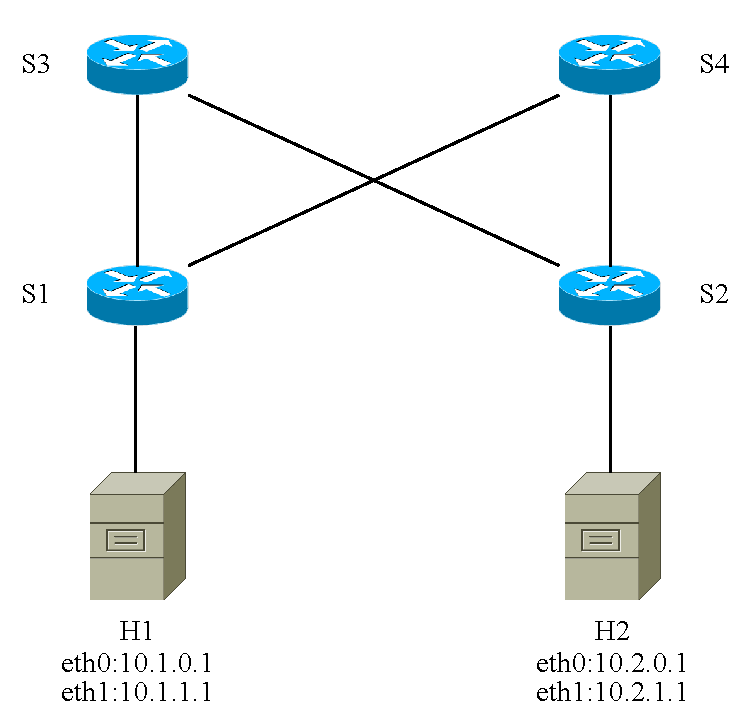
\includegraphics[autoebb, width=250pt]{./img/pair_problem.pdf}
    \caption{Techinical problem of creating subflow without complete paired IP
    addressses}
    %\ecaption{The control loop in DCTCP}
    \label{fig:mptcp_pair}
    \end{center}
\end{figure}

\section{Incast問題に対する考察}
データセンターが抱える性能障害の一つにIncast問題がある. 
これは, 一つのインタフェースに大量のショートフローが同時に集中することにより遅延が生じるという, データセンターでの並列分散処理が生み出す特有の問題である. 
今のMPTCP実装では, サイズの小さい通信には複数経路を用いずに一つの経路だけで通信が完了するため, 今回の提案手法のような経路切替手法は有効に働かない. 
例えば, エンドノード間の通信経路が3本存在している時には, SLに2経路, LLに1経路割り当て,
ラウンドロビンやハッシュベースを用いた負荷分散手法が有効であると考える. 
このような従来のECMPによるアプローチと比べ, レーンモデルによるフローの区別を行うことで, ショートフローに対してのみロードバランスすれば良いため,
Fig.\ref{fig:repflow_scenario}のような性能障害が起きないと考える. 

実際。。。(グラフを示す)



\chapter{結論}
\label{chapter:conclusion}

\section{今後の課題}


\chapter*{発表文献}

\section*{国内会議(査読あり)}
\begin{enumerate}
\bibitem{mywork_2}{藤居 翔吾, 田崎 創, 関谷 勇司, "MultiPath TCP
適用時のデータセンターネットワークでのフローサイズが与える影響に関する一考察", インターネットカンファレンス2014}
\end{enumerate}
\section*{国内会議(査読なし)}
\begin{enumerate}
\bibitem{mywork_1}{藤居 翔吾, 田崎 創, 関谷 勇司, "データセンター環境におけるショートフロー通信改善手法の一提案", 電子情報通信学会, 信学技法, vol. 113, no. 364,
IA2013-65, pp. 47-52, 2013.}
\end{enumerate}

\section*{受賞}
\begin{enumerate}
\bibitem{mywork_1}{学生研究奨励賞:藤居 翔吾, 田崎 創, 関谷 勇司, "データセンター環境におけるショートフロー通信改善手法の一提案",
電子情報通信学会, 信学技法, vol. 113, no. 364, IA2013-65, pp. 47-52, 2013.}
\bibitem{mywork_2}{学生奨励賞:藤居 翔吾, 田崎 創, 関谷 勇司, "MultiPath TCP
適用時のデータセンターネットワークでのフローサイズが与える影響に関する一考察", インターネットカンファレンス2014}
\end{enumerate}


\chapter*{謝辞}


本研究および大学院修士課程2年間の生活においてご指導ご鞭撻していただいた東京大学の関谷勇司准教授と田崎創特任講師に深く感謝いたします.
また,
本研究を進めるにあたり多くの建設的な意見を与えてくださった東京大学の若原恭教授,中山雅哉准教授,小川剛史准教授,妙中雄三助教,宮本大輔助教に心より感謝いたします. 研究室での生活においては,Jia Xiazhou氏をはじめ,多くの心優しい同期,先輩,後輩に恵まれ,大変充実した2年間を送ることができました.
ここに感謝の意を表します.
最後に,長い学生生活を支えてくださった両親,兄弟に深く深く心より感謝を致します.


\vspace{1cm}
\begin{thebibliography}{99}
\bibitem{IBM_rep}{日本アイ・ビー・エム株式会社. IBM 第1章
大容量データのバックアップ,
\url{http://www-06.ibm.com/systems/jp/storage/column/backup/01.html}}
\bibitem{amazon}{Jim Liddle. Amazon found every 100ms of latency cost them 1\%
in sales, August 2008.
\url{http://blog.gigaspaces.com/amazon-found-every-100ms-of-latency-cost-them-1-in-sales/}}

\bibitem{customer_impact}{R. Kohavi et al. Practical Guide to Controlled
Experiments on theWeb: Listen to Your Customers not to the HiPPO. KDD, 2007.}
\bibitem{requirement}{J. Hamilton. On designing and deploying Internet-scale
services. In USENIX LISA, 2007.}
\bibitem{presto}{Facebook. Presto: Interacting with petabytes
of data at Facebook,
\url{https://www.facebook.com/notes/facebook-engineering/presto-interacting-with-petabytes-of-data-at-facebook/10151786197628920}}
\bibitem{mapreduce}{Dean, Jeffrey, and Sanjay
Ghemawat. "MapReduce: simplified data processing on large clusters." Communications of the ACM 51.1 (2008): 107-113.}
\bibitem{fattree}{Al-Fares, Mohammad, Alexander L oukissas, and Amin Vahdat. "A
scalable, commodity data center network architecture." ACM SIGCOMM Computer
Communication Review. Vol. 3}
\bibitem{dctcp}{Alizadeh, Mohammad, et al. "Data center tcp (dctcp)." ACM SIGCOMM Computer Communication Review 40.4 (2010): 63-74.}
\bibitem{improving}{Raiciu, Costin, et al. "Improving datacenter performance and
robustness with multipath TCP." ACM SIGCOMM Computer Communication Review. Vol. 41. No. 4. ACM, 2011.}
\bibitem{detail}{Zats, David, et al. "DeTail: Reducing the flow completion time
tail in datacenter networks." ACM SIGCOMM Computer Communication Review 42.4 (2012): 139-150.}
\bibitem{p_fab}{Alizadeh, Mohammad, et al. "pfabric: Minimal near-optimal datacenter transport." Proceedings of the ACM SIGCOMM 2013 conference on SIGCOMM. ACM, 2013.}
\bibitem{click}{Kohler, Eddie, et al. "The Click modular router." ACM
Transactions on Computer Systems (TOCS) 18.3 (2000): 263-297.}
\bibitem{mptcp}{Ford, Alan, et al. TCP Extensions for Multipath Operation with
Multiple Addresses: draft-ietf-mptcp-multiaddressed-03. No. Internet draft (draft-ietf-mptcp-multiaddressed-07). Roke Manor, 2011.}
\bibitem{traffic}{Benson, Theophilus, Aditya Akella, and David A. Maltz.
"Network traffic characteristics of data centers in the wild." Proceedings of the 10th ACM SIGCOMM conference on Internet measurement. ACM, 2010.}
\bibitem{NAPI}{J. Salim, When NAPI Comes to Town, Proceedings of Linux 2005
Conference, UK, August 2005.}
\bibitem{RSS}{Microsoft corporation. scalable networking with rss, 2005.}
\bibitem{RFS}{Herbert, T. rfs: receive flow steering, september 2010.
http://lwn.net/Articles/381955/.} 
\bibitem{RPS}{Herbert, T. rps: receive packet steering, september 2010.
\url{http://lwn.net/Articles/361440/.}}
\bibitem{mptcp_linux}{ip networking lab「MultiPath TCP - Linux Kernel
implementation」\url{http://mptcp.info.ucl.ac.be/}} 
\bibitem{rtt}{Vasudevan, Vijay, et al. "Safe and effective fine-grained TCP
retransmissions for datacenter communication." ACM SIGCOMM Computer Communication Review. Vol. 39. No. 4. ACM, 2009.}
\bibitem{mptcp_ana}{藤居 翔吾, 田崎 創, 関谷 勇司, "MultiPath TCP
適用時のデータセンターネットワークでのフローサイズが与える影響に関する一考察", 電子情報通信学会, 信学技法, vol. 113, no. 364,
IA2013-65, pp. 47-52, 2013.}
\bibitem{mptcp_ana2}{藤居翔吾, 田崎創, 関谷勇司, "MultiPath TCP 適用時のデータセンター
ネットワークでのフローサイズが与える影響に関する一考察", 日本ソフトウェア科学会研究会資料シリーズ No.74 ISSN1341-870X,
インターネットコンファレス2014論文集, pp33-42 } 
\bibitem{flexible}{P. Agarwal, B. Kwan, and L. Ashvin. Flexible buffer allocation entities for
traffic aggregate containment. US Patent 20090207848, August 2009.}
\bibitem{synchro}{S. Floyd and V. Jacobson. The synchronization of periodic routing messages.
IEEE/ACM ToN, 1994.}
\bibitem{balia}{A. Walid, et al. Balanced Linked Adaptation Congestion Control
Algorithm for MPTCP draft-walid-mptcp-congestion-control-00, 2014.}
\bibitem{tcpdump}{tcpdump, \url{http://www.tcpdump.org/}}
\bibitem{intel}{intel,
\url{http://www.intel.com/content/www/us/en/network-adapters/gigabit-network-adapters/ethernet-server-adapters.html}}
\bibitem{bottleneck}{Lu, Guohan, et al. "Using cpu as a traffic co-processing
unit in commodity switches." Proceedings of the first workshop on Hot topics in software defined networks. ACM, 2012.}
\bibitem{sctp}{R. Stewart. Stream Control Transmission Protocol. RFC 4960
(Proposed Standard), September 2007. Updated by RFCs 6096, 6335. }
\bibitem{cmt_1}{Iyengar, Janardhan R., Paul D. Amer, and Randall Stewart.
"Concurrent multipath transfer using SCTP multihoming over independent end-to-end paths." Networking, IEEE/ACM Transactions on 14.5 (2006): 951-964.}
\bibitem{cmt_2}{Iyengar, Janardhan, et al. "Concurrent multipath transfer using
SCTP multihoming." SPECTS 2004 (2004).}
\bibitem{lacp}{IEEE Standards Association. "IEEE 802.3 LAN/MAN CSMA/CD Access
Method." (2008).}
\bibitem{lacp_problem}{Fukunaga, Takafumi, and Hidenori Umeno. "Implementation
and evaluation of improvement in parallel processing performance on the cluster using small-scale SMP PCs." IEEJ Transactions on Electronics, Information and Systems 128 (2008): 1842-1851.}
\bibitem{arp}{Umeshima S, Higaki H. Extended ARP for high-per-
formance LAN communications with multiple kinds
of NICs. 2003-DSM-029, Vol. 2003, No. 38, p 31–36,
2003.}
\bibitem{oldi}{Meisner, David, et al. "Power management of online data-intensive
services." Computer Architecture (ISCA), 2011 38th Annual International Symposium on. IEEE, 2011.}
\bibitem{incast}{Chen, Yanpei, et al. "Understanding TCP incast throughput
collapse in datacenter networks." Proceedings of the 1st ACM workshop on Research on enterprise networking. ACM, 2009.}
\bibitem{desynchro}{Floyd, Sally, and Van Jacobson. "The synchronization of
periodic routing messages." Networking, IEEE/ACM Transactions on 2.2 (1994): 122-136.}
\bibitem{memory}{Iyer, Sundar, Ramana Rao Kompella, and N. McKeowa. "Analysis of
a memory architecture for fast packet buffers." High Performance Switching and Routing, 2001 IEEE Workshop on. IEEE, 2001.}
\bibitem{websearch}{Barroso, Luiz André, Jeffrey Dean, and Urs Holzle. "Web
search for a planet: The Google cluster architecture." Micro, Ieee 23.2 (2003): 22-28.}
\bibitem{d3}{Wilson, Christo, et al. "Better never than late: Meeting deadlines
in datacenter networks." ACM SIGCOMM Computer Communication Review. Vol. 41. No. 4. ACM, 2011.}
\bibitem{d2tcp}{Vamanan, Balajee, Jahangir Hasan, and T. N. Vijaykumar.
"Deadline-aware datacenter tcp (d2tcp)." ACM SIGCOMM Computer Communication Review 42.4 (2012): 115-126.}
\bibitem{key-value1}{Beaver, Doug, et al. "Finding a Needle in Haystack:
Facebook's Photo Storage." OSDI. Vol. 10. 2010.}
\bibitem{key-value2}{Hastorun, Deniz, et al. "Dynamo: Amazon’s highly available
key-value store." In Proc. SOSP. 2007.}
\bibitem{dryad}{Isard, Michael, et al. "Dryad: distributed data-parallel
programs from sequential building blocks." ACM SIGOPS Operating Systems Review. Vol. 41. No. 3. ACM, 2007.}
\bibitem{repflow}{Liu, Shuhao, et al. "RepFlow on node. js: Cutting Tail Latency
in Data Center Networks at the Applications Layer." arXiv preprint arXiv:1407.1239 (2014).}
\bibitem{vl2}{Greenberg, Albert, et al. "VL2: a scalable and flexible data
center network." ACM SIGCOMM Computer Communication Review. Vol. 39. No. 4. ACM, 2009.}
\bibitem{devoflow}{Curtis, Andrew R., et al. "Devoflow: scaling flow management
for high-performance networks." ACM SIGCOMM Computer Communication Review. Vol. 41. No. 4. ACM, 2011.}
\bibitem{clos}{Clos, Charles. "A Study of Non‐Blocking Switching Networks." Bell
System Technical Journal 32.2 (1953): 406-424.}
\bibitem{bpr}{U.S. Department of Commerce, Bureau of Public Roads(1964),
Traffic Assignment Manual}
\bibitem{davidson}{Davidson, K. B. "A flow travel time relationship for use in
transportation planning." Australian Road Research Board (ARRB) Conference, 3rd, 1966, Sydney. Vol. 3. No. 1. 1966.}
\bibitem{ns3}{Tazaki, Hajime, et al. "Direct code execution: Revisiting library
os architecture for reproducible network experiments." Proceedings of the ninth ACM conference on Emerging networking experiments and technologies. ACM, 2013.}
\bibitem{crossbar}{McKeown, Nick. "A fast switched backplane for a
gigabit switched router." Business Communications Review 27.12 (1997): 1-30.}
\bibitem{delay}{Priority flow control: Build reliable layer 2 infrastructure.
\url{http://www.cisco.com/en/US/prod/collateral/switches/
ps9441/ps9670/white_paper_c11-542809.pdf}}
\bibitem{pdq}{Hong, Chi-Yao, Matthew Caesar, and P. Godfrey. "Finishing flows
quickly with preemptive scheduling." ACM SIGCOMM Computer Communication Review 42.4 (2012): 127-138.}
\bibitem{survey}{Liu, Shuhao, Hong Xu, and Zhiping Cai. "Low latency datacenter
networking: A short survey." arXiv preprint arXiv:1312.3455 (2013).}
\bibitem{hull}{Alizadeh, Mohammad, et al. "Less is more: trading a little
bandwidth for ultra-low latency in the data center." Proceedings of the 9th USENIX conference on Networked Systems Design and Implementation. USENIX Association, 2012.}
\bibitem{dibs}{Zarifis, Kyriakos, et al. "DIBS: just-in-time congestion
mitigation for data centers." Proceedings of the Ninth European Conference on Computer Systems. ACM, 2014.}
\bibitem{fastlane}{Zats, David, et al. FastLane: An agile congestion signaling
mechanism for improving datacenter performance. No. UCB/EECS-2013-113. CALIFORNIA UNIV BERKELEY DEPT OF ELECTRICAL ENGINEERING AND COMPUTER SCIENCE, 2013.}
\bibitem{cp}{Cheng, Peng, et al. "Catch the whole lot in an action: Rapid
precise packet loss notification in data centers." Proc. USENIX NSDI. 2014.}
\bibitem{mcp}{Chen, Li, et al. "Towards minimal-delay deadline-driven data
center tcp." Proceedings of the Twelfth ACM Workshop on Hot Topics in Networks. ACM, 2013.}
\bibitem{bcube}{Guo, Chuanxiong, et al. "BCube: a high performance,
server-centric network architecture for modular data centers." ACM SIGCOMM Computer Communication Review 39.4 (2009): 63-74.}
\bibitem{cong}{Raiciu, C., M. Handley, and D. Wischik. "Coupled congestion
control for multipath transport protocols." draft-ietf-mptcp-congestion-01 (work in progress) (2011).}
\bibitem{RTT_est}{Jacobsson, Krister, et al. "Round trip time estimation
in communication networks using adaptive kalman filtering." (2004).}
\bibitem{queue_delay}{Angrisani, Leopoldo, et al. "Measurement of processing and
queuing delays introduced by an open-source router in a single-hop network."
Instrumentation and Measurement, IEEE Transactions on 55.4 (2006): 1065-1076.}
\bibitem{trouble}{DEAN, J. Software engineering advice from building large-scale distributed systems. http://research.google.com/people/jeff/stanford-295-talk.pdf.
}
\bibitem{openflow}{McKeown, Nick, et al. "OpenFlow: enabling innovation in
campus networks." ACM SIGCOMM Computer Communication Review 38.2 (2008): 69-74.}
\end{thebibliography}
\clearpage
\def\thesection{}
\def\thesubsection{\Alph{subsection}}
\def\thesection{付録\Alph{section}}
\setcounter{subsection}{0}
\appendix
\section{リンクパフォーマンス関数:Davidson関数}
リンクパフォーマンス関数は, ネットワークを構成する個々のリンクのサービス水準をリンク交通量とリンク属性の関数として表したものである. 
本研究では, リンクのサービス水準には, フロー完結時間(旅行時間)を用いている. 
リンクパフォーマンス関数は, 狭義の増加関数である必要があり, このことは待ち行列理論を用いて説明することができる. 

今, M/M/1($\infty$)の待ち行列理論を考える. 
この時, 到着率$\lambda$, サービス率$\mu$を用いて利用率$\rho$は以下のように表される. 

\begin{equation}
\label{utilization}
\rho = \frac{\lambda}{\mu}
\end{equation}

この利用率$\rho$と平均サービス時間$T_s$を用いて, 待ち時間$T_w$は以下のように表される. 
\begin{equation}
\label{traffic}
T_w = \frac{\rho}{1-\rho} \times T_s
\end{equation}

次にあるリンクにおけるフロー完結時間$t$を導出する. 
このリンクにおいて, 他のフローが存在しない時のフロー完結時間を$t_0$とする. 
この時, 遅れのパラメータ$J(>0)$と式\ref{utilization}, \ref{traffic}を用いて以下のように表すことができる. 
\begin{equation}
\label{delay}
J t_0 \frac{\rho}{1-\rho} = J t_0 \frac{q}{C-q} 
\end{equation}
ここで, $q$はリンク利用率, $C$はリンク容量である.
これにより, フロー完結時間$t(q)$は次のように定義される. 
\begin{eqnarray}
t(q) = t_{0} + J t_{0} \frac{\rho}{1-\rho} = t_{0}\Bigl\{ 1 + J \bigl(
\frac{q}{C-q} \bigr) \Bigr\}
\end{eqnarray}


\end{document}